\documentclass[11pt,a4paper]{article}

% Packages
\usepackage[utf8]{inputenc}
\usepackage[T1]{fontenc}
\usepackage{amsmath,amssymb,amsthm}
\usepackage{algorithm}
\usepackage{algpseudocode}
\usepackage{booktabs}
\usepackage{graphicx}
\usepackage{hyperref}
\usepackage{listings}
\usepackage{xcolor}
\usepackage{tikz}
\usetikzlibrary{shapes.geometric,arrows.meta,positioning}
\usepackage{geometry}

\geometry{margin=1in}

% Code listing style
\lstdefinestyle{rust}{
    language=C,
    basicstyle=\ttfamily\small,
    keywordstyle=\color{blue}\bfseries,
    commentstyle=\color{gray},
    stringstyle=\color{red},
    numbers=left,
    numberstyle=\tiny\color{gray},
    breaklines=true,
    frame=single,
    showstringspaces=false
}

\lstdefinestyle{solidity}{
    language=C,
    basicstyle=\ttfamily\small,
    keywordstyle=\color{purple}\bfseries,
    commentstyle=\color{gray},
    stringstyle=\color{orange},
    numbers=left,
    numberstyle=\tiny\color{gray},
    breaklines=true,
    frame=single
}

% Theorem environments
\newtheorem{theorem}{Theorem}[section]
\newtheorem{lemma}[theorem]{Lemma}
\newtheorem{definition}[theorem]{Definition}
\newtheorem{property}[theorem]{Property}

% Title
\title{\textbf{Proof of AI: An Open Protocol for Decentralized AI Mining}\\[0.5em]
\large Bitcoin-Inspired Token Economics with Quantum-Safe Security}

\author{
Lux Network Foundation\thanks{Technical Contact: team@lux.network} \\
Hanzo AI\thanks{AI Infrastructure: team@hanzo.ai} \\
Zoo Labs Foundation\thanks{DeSci Research: team@zoo.ngo}
}

\date{Version 1.0 --- December 2025}

\begin{document}

\maketitle

\begin{abstract}
This paper presents \textbf{Proof of AI (PoAI)}, an open protocol enabling anyone with GPU compute to mine AI tokens across the Lux ecosystem. Inspired by Bitcoin's elegant simplicity, PoAI establishes a fixed supply of 1 billion AI tokens per chain, with mining rewards halving on a schedule aligned with Bitcoin's halvings. The protocol leverages NVIDIA's NVTrust for hardware attestation, ML-DSA quantum-safe signatures for long-term security, and Quasar consensus for instant finality. Unlike traditional mining, PoAI rewards \textit{useful} AI compute---inference, training, and research---while preventing double-spend through cryptographic chain-binding. The Teleport bridge enables seamless cross-chain liquidity across Hanzo EVM, Zoo EVM, and Lux C-Chain, with a novel global supply cap that only increases as new chains join the network.
\end{abstract}

\tableofcontents
\newpage

% Include sections
\section{Introduction}
\label{sec:introduction}

\subsection{The Vision: Open AI for Everyone}

The artificial intelligence revolution has been captured by centralized corporations. Access to frontier models requires expensive API subscriptions, training compute is controlled by hyperscalers, and the economic benefits of AI accrue to shareholders rather than contributors.

\textbf{Proof of AI (PoAI)} democratizes this landscape by creating an open protocol where:

\begin{enumerate}
    \item \textbf{Anyone with a GPU can participate} --- from a single RTX 4090 to data center H100 clusters
    \item \textbf{Miners earn AI tokens} for providing useful compute (inference, training, research)
    \item \textbf{Users pay for services} with AI tokens, creating a self-sustaining economy
    \item \textbf{Supply is fixed and predictable} --- 1 billion tokens per chain, halving like Bitcoin
    \item \textbf{Cross-chain liquidity} enables tokens to flow freely via Teleport
\end{enumerate}

\subsection{Design Philosophy}

PoAI draws inspiration from Bitcoin's elegant simplicity while adapting to AI compute requirements:

\begin{center}
\begin{tabular}{lll}
\toprule
\textbf{Aspect} & \textbf{Bitcoin} & \textbf{Proof of AI} \\
\midrule
Work & SHA-256 hashing & AI inference/training \\
Supply & 21M BTC & 1B AI per chain \\
Halving & Every 210,000 blocks & Every 210,000 blocks \\
Finality & ~60 minutes (6 confirms) & ~500ms (Quasar) \\
Signatures & ECDSA & ML-DSA (quantum-safe) \\
Hardware & ASICs & GPUs with NVTrust \\
\bottomrule
\end{tabular}
\end{center}

\subsection{Core Innovation: Chain-Bound AI Work}

The fundamental innovation of PoAI is \textbf{chain-binding}: each unit of AI work is cryptographically committed to a specific chain \textit{before} the compute runs. This prevents ``copy-paste mining'' where the same work is submitted to multiple chains.

\begin{definition}[Chain-Bound Work]
A unit of AI work $W$ is chain-bound if and only if:
\begin{enumerate}
    \item The target chain ID $c$ is included in the work context before computation
    \item The GPU's NVTrust enclave signs a receipt including $c$
    \item Each chain maintains a spent set preventing double-minting
\end{enumerate}
\end{definition}

\subsection{Ecosystem Overview}

PoAI operates across three primary chains in the Lux ecosystem:

\begin{center}
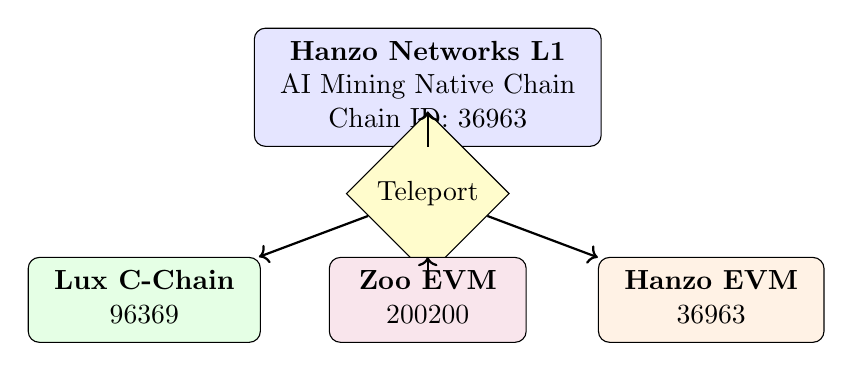
\begin{tikzpicture}[scale=0.9]
    % Hanzo L1
    \node[draw, rectangle, rounded corners, fill=blue!10, minimum width=4cm, minimum height=1.5cm] (hanzo) at (0,3) {
        \begin{tabular}{c}
        \textbf{Hanzo Networks L1} \\
        AI Mining Native Chain \\
        Chain ID: 36963
        \end{tabular}
    };

    % Teleport
    \node[draw, diamond, fill=yellow!20, minimum width=1.5cm] (teleport) at (0,1.5) {Teleport};

    % EVM Chains
    \node[draw, rectangle, rounded corners, fill=green!10, minimum width=2.5cm, minimum height=1cm] (lux) at (-4,0) {
        \begin{tabular}{c}
        \textbf{Lux C-Chain} \\
        96369
        \end{tabular}
    };

    \node[draw, rectangle, rounded corners, fill=purple!10, minimum width=2.5cm, minimum height=1cm] (zoo) at (0,0) {
        \begin{tabular}{c}
        \textbf{Zoo EVM} \\
        200200
        \end{tabular}
    };

    \node[draw, rectangle, rounded corners, fill=orange!10, minimum width=2.5cm, minimum height=1cm] (hanzo_evm) at (4,0) {
        \begin{tabular}{c}
        \textbf{Hanzo EVM} \\
        36963
        \end{tabular}
    };

    % Arrows
    \draw[->, thick] (hanzo) -- (teleport);
    \draw[->, thick] (teleport) -- (lux);
    \draw[->, thick] (teleport) -- (zoo);
    \draw[->, thick] (teleport) -- (hanzo_evm);
\end{tikzpicture}
\end{center}

\subsection{Document Structure}

This paper is organized as follows:

\begin{itemize}
    \item \textbf{Section~\ref{sec:tokenomics}}: Token economics, supply schedule, halving mechanism
    \item \textbf{Section~\ref{sec:proof-of-ai}}: Proof of AI consensus and reward calculation
    \item \textbf{Section~\ref{sec:nvtrust}}: NVTrust chain-binding and double-spend prevention
    \item \textbf{Section~\ref{sec:difficulty}}: Difficulty adjustment algorithm
    \item \textbf{Section~\ref{sec:payments}}: Market dynamics and payment for services
    \item \textbf{Section~\ref{sec:multi-chain}}: Multi-chain mining with Teleport
    \item \textbf{Section~\ref{sec:evm-contracts}}: EVM contracts for reward claiming
    \item \textbf{Section~\ref{sec:security}}: Security analysis and quantum safety
    \item \textbf{Section~\ref{sec:conclusion}}: Conclusion and future work
    \item \textbf{Section~\ref{sec:zkproofs}}: Shielded mining via zero-knowledge proofs
\end{itemize}

\section{Token Economics}
\label{sec:tokenomics}

\subsection{Fixed Supply Per Chain}

Each chain in the PoAI ecosystem has a fixed maximum supply of \textbf{1 billion AI tokens}:

\begin{equation}
\text{Supply}_{\text{chain}} = 1,000,000,000 \text{ AI}
\end{equation}

\begin{definition}[Global Supply]
The global AI supply $S_{\text{global}}$ increases only as new chains join the network:
\begin{equation}
S_{\text{global}} = \sum_{i=1}^{n} S_{\text{chain}_i} = n \times 10^9 \text{ AI}
\end{equation}
where $n$ is the number of active chains.
\end{definition}

\begin{center}
\begin{tabular}{lcc}
\toprule
\textbf{Chain} & \textbf{Chain ID} & \textbf{Max Supply} \\
\midrule
Hanzo EVM & 36963 & 1,000,000,000 AI \\
Zoo EVM & 200200 & 1,000,000,000 AI \\
Lux C-Chain & 96369 & 1,000,000,000 AI \\
\midrule
\textbf{Total (3 chains)} & --- & \textbf{3,000,000,000 AI} \\
\bottomrule
\end{tabular}
\end{center}

\subsection{Bitcoin-Aligned Halving Schedule}

Mining rewards halve every 210,000 blocks, perfectly aligned with Bitcoin's halving schedule:

\begin{equation}
R_{\text{block}}(h) = R_0 \times 2^{-\lfloor h / 210000 \rfloor}
\end{equation}

where:
\begin{itemize}
    \item $R_{\text{block}}(h)$ = reward per block at height $h$
    \item $R_0$ = initial block reward
    \item $\lfloor \cdot \rfloor$ = floor function
\end{itemize}

\subsubsection{Initial Block Reward Calculation}

To distribute 1 billion tokens following Bitcoin's halving schedule:

\begin{equation}
\sum_{i=0}^{\infty} 210000 \times R_0 \times 2^{-i} = 210000 \times R_0 \times 2 = 1,000,000,000
\end{equation}

Solving for $R_0$:
\begin{equation}
R_0 = \frac{1,000,000,000}{420,000} = 2,380.95 \text{ AI per block}
\end{equation}

Rounding to $R_0 = 2,381$ AI per block.

\subsection{Halving Timeline}

With target block time of 2 seconds (Quasar consensus):

\begin{center}
\begin{tabular}{cccc}
\toprule
\textbf{Era} & \textbf{Block Range} & \textbf{Reward} & \textbf{Est. Date} \\
\midrule
1 & 0 -- 209,999 & 2,381 AI & Genesis -- +4.8 days \\
2 & 210,000 -- 419,999 & 1,190.5 AI & +4.8 days -- +9.7 days \\
3 & 420,000 -- 629,999 & 595.25 AI & +9.7 days -- +14.5 days \\
4 & 630,000 -- 839,999 & 297.62 AI & +14.5 days -- +19.4 days \\
\vdots & \vdots & \vdots & \vdots \\
32 & 6,510,000+ & $<$1 AI & +75 days \\
\bottomrule
\end{tabular}
\end{center}

\textbf{Note:} With 2-second blocks, halving occurs approximately every 4.86 days rather than Bitcoin's 4 years. For longer-term distribution, the block time can be adjusted or halving interval increased.

\subsection{Supply Distribution}

\begin{theorem}[Total Mined Supply]
The total supply $S$ mined after $n$ complete halving eras is:
\begin{equation}
S(n) = R_0 \times 210000 \times (2 - 2^{1-n})
\end{equation}
which approaches $1B$ as $n \to \infty$.
\end{theorem}

\begin{proof}
Geometric series:
$S = \sum_{i=0}^{n-1} 210000 \times R_0 \times 2^{-i} = 210000 \times R_0 \times \frac{1 - 2^{-n}}{1 - 2^{-1}} = 420000 \times R_0 \times (1 - 2^{-n})$
\end{proof}

\subsection{Token Utility}

AI tokens serve multiple functions in the ecosystem:

\begin{enumerate}
    \item \textbf{Payment for AI Services}: Users pay miners for inference, training, fine-tuning
    \item \textbf{Governance}: Token holders vote on protocol parameters
    \item \textbf{Staking}: Miners stake AI to increase reward priority
    \item \textbf{Cross-Chain Liquidity}: Teleport enables DeFi integration
    \item \textbf{Research Funding}: Treasury contributions fund open AI research
\end{enumerate}

\subsection{Treasury Allocation}

Each chain allocates a portion of mining rewards to research and development:

\begin{equation}
\text{Treasury}(R) = 0.02 \times R
\end{equation}

A 2\% contribution from all mining rewards funds:
\begin{itemize}
    \item Open-source model development
    \item Protocol security audits
    \item Community grants
    \item Infrastructure maintenance
\end{itemize}

\subsection{Atomic Units}

Like Bitcoin's satoshis, AI tokens have atomic units called \textbf{neurons}:

\begin{equation}
1 \text{ AI} = 10^{18} \text{ neurons}
\end{equation}

This allows for precise micropayments for AI inference:
\begin{itemize}
    \item 1 token generation $\approx$ 1,000 neurons
    \item 1 image generation $\approx$ 100,000 neurons
    \item 1 minute of speech recognition $\approx$ 10,000 neurons
\end{itemize}

\section{Proof of AI Consensus}
\label{sec:proof-of-ai}

\subsection{Overview}

Proof of AI (PoAI) is a consensus mechanism that rewards \textit{useful} AI compute rather than wasteful hash computation. Miners earn AI tokens by:

\begin{enumerate}
    \item Providing inference services (LLM, vision, audio)
    \item Contributing training compute for model improvement
    \item Running research workloads for scientific discovery
\end{enumerate}

\subsection{Work Types}

\begin{definition}[AI Work Types]
PoAI recognizes three categories of useful work:
\begin{align}
W_{\text{inference}} &= \text{tokens\_processed} \times \text{model\_complexity} \\
W_{\text{training}} &= \text{flops} \times \text{batch\_size} \times \text{gradient\_steps} \\
W_{\text{research}} &= \text{compute\_hours} \times \text{job\_complexity}
\end{align}
\end{definition}

\subsection{Reward Calculation}

The reward for a unit of AI work is:

\begin{equation}
R = R_{\text{base}} \times W \times D^{-1} \times M_{\text{GPU}} \times M_{\text{uptime}}
\end{equation}

where:
\begin{itemize}
    \item $R_{\text{base}}$ = base reward per compute unit
    \item $W$ = work units (tokens, FLOPs, etc.)
    \item $D$ = current network difficulty
    \item $M_{\text{GPU}}$ = GPU tier multiplier
    \item $M_{\text{uptime}}$ = uptime bonus (0.9--1.1)
\end{itemize}

\subsubsection{GPU Tier Multipliers}

\begin{center}
\begin{tabular}{lccc}
\toprule
\textbf{GPU Model} & \textbf{NVTrust} & \textbf{Trust Score} & \textbf{Multiplier} \\
\midrule
GB200 & Full + TEE-I/O & 100 & 1.5 \\
B200 & Full + TEE-I/O & 100 & 1.5 \\
B100 & Full + TEE-I/O & 100 & 1.5 \\
H200 & Full & 95 & 1.3 \\
H100 & Full & 95 & 1.3 \\
RTX PRO 6000 & Basic & 85 & 1.1 \\
RTX 5090 & Software only & 60 & 0.8 \\
RTX 4090 & Software only & 60 & 0.8 \\
\bottomrule
\end{tabular}
\end{center}

\subsection{Work Proof Structure}

Each mining proof contains:

\begin{lstlisting}[style=rust]
pub struct AIWorkProof {
    // Identity
    pub miner_pubkey: [u8; 1952],     // ML-DSA-65 public key
    pub device_id: [u8; 32],          // GPU hardware ID

    // Chain binding
    pub chain_id: u64,                // Target chain (36963/200200/96369)
    pub nonce: [u8; 32],              // Unique per job
    pub timestamp: u64,               // Unix timestamp

    // Work specification
    pub model_hash: [u8; 32],         // BLAKE3 of model weights
    pub input_hash: [u8; 32],         // BLAKE3 of input data
    pub output_hash: [u8; 32],        // BLAKE3 of output

    // Work metrics
    pub work_type: WorkType,
    pub compute_units: u64,
    pub tokens_processed: u64,
    pub flops: u64,

    // Attestation
    pub nvtrust_signature: Vec<u8>,   // NVTrust enclave signature
    pub spdm_evidence: Vec<u8>,       // GPU firmware measurement

    // Miner signature
    pub signature: Vec<u8>,           // ML-DSA signature over proof
}
\end{lstlisting}

\subsection{Validation Rules}

A proof is valid if and only if:

\begin{enumerate}
    \item \textbf{Signature Valid}: ML-DSA signature verifies against miner pubkey
    \item \textbf{NVTrust Valid}: NVTrust signature chains to NVIDIA root CA
    \item \textbf{Chain Bound}: $\text{proof.chain\_id} = \text{current\_chain\_id}$
    \item \textbf{Not Spent}: $\text{hash}(\text{device\_id} \| \text{nonce} \| \text{chain\_id}) \notin \text{SpentSet}$
    \item \textbf{Fresh}: $|\text{timestamp} - \text{block\_time}| < \text{PROOF\_EXPIRY}$
    \item \textbf{Meets Difficulty}: Work exceeds current difficulty target
\end{enumerate}

\begin{algorithm}
\caption{ValidateAIWorkProof}
\begin{algorithmic}[1]
\Require AIWorkProof $P$, ChainState $S$
\Ensure Boolean validity
\State \textbf{verify} $P.\text{signature}$ against $P.\text{miner\_pubkey}$
\State \textbf{verify} $P.\text{nvtrust\_signature}$ against NVIDIA root
\If{$P.\text{chain\_id} \neq S.\text{chain\_id}$}
    \State \Return \textbf{false} \Comment{Wrong chain binding}
\EndIf
\State $\text{work\_id} \gets \text{BLAKE3}(P.\text{device\_id} \| P.\text{nonce} \| P.\text{chain\_id})$
\If{$\text{work\_id} \in S.\text{spent\_set}$}
    \State \Return \textbf{false} \Comment{Double-spend attempt}
\EndIf
\If{$|P.\text{timestamp} - S.\text{block\_time}| > \text{PROOF\_EXPIRY}$}
    \State \Return \textbf{false} \Comment{Proof expired}
\EndIf
\State \textbf{verify} $P.\text{compute\_units} \geq S.\text{difficulty\_target}$
\State \Return \textbf{true}
\end{algorithmic}
\end{algorithm}

\subsection{Block Structure}

Blocks contain aggregated AI work proofs:

\begin{lstlisting}[style=rust]
pub struct AIBlock {
    // Header
    pub height: u64,
    pub prev_hash: [u8; 32],
    pub merkle_root: [u8; 32],        // Merkle root of proofs
    pub state_root: [u8; 32],         // State trie root
    pub timestamp: u64,
    pub difficulty: u64,

    // Proofs
    pub proofs: Vec<AIWorkProof>,     // Up to MAX_PROOFS_PER_BLOCK
    pub total_work: u64,              // Sum of all work units
    pub total_rewards: u128,          // Sum of all rewards

    // Consensus
    pub proposer: [u8; 1952],         // Block proposer pubkey
    pub quasar_signature: Vec<u8>,    // Quasar consensus signature
}
\end{lstlisting}

\subsection{Integration with Quasar Consensus}

PoAI integrates with Quasar for instant finality:

\begin{enumerate}
    \item \textbf{Proposer Selection}: Weighted by staked AI tokens + cumulative work
    \item \textbf{Finality}: 2-round BFT with $\frac{2}{3}$ supermajority
    \item \textbf{Block Time}: 500ms target (sub-second user experience)
    \item \textbf{Signatures}: ML-DSA for quantum safety
\end{enumerate}

\begin{property}[Finality Guarantee]
Under Quasar consensus with $n$ validators and at most $f < n/3$ Byzantine:
\begin{itemize}
    \item \textbf{Safety}: No two honest validators finalize conflicting blocks
    \item \textbf{Liveness}: If $\geq 2n/3$ validators are honest, blocks finalize within 2 rounds
\end{itemize}
\end{property}

\section{NVTrust Chain-Binding}
\label{sec:nvtrust}

\subsection{Double-Spend Prevention}

The fundamental security challenge in multi-chain AI mining is preventing ``copy-paste mining''---submitting the same work to multiple chains for multiple rewards. PoAI solves this via \textbf{chain-binding}: cryptographically committing each unit of work to a specific chain before computation begins.

\begin{definition}[Double-Spend Attack]
An attacker performs work $W$ once but claims rewards on chains $C_1, C_2, \ldots, C_n$ by submitting the same or slightly modified proofs.
\end{definition}

\begin{theorem}[Double-Spend Resistance]
Under chain-binding with NVTrust attestation, the probability of a successful double-spend is:
\begin{equation}
P(\text{double-spend}) \leq \text{negl}(\lambda)
\end{equation}
where $\lambda$ is the security parameter (256-bit for BLAKE3).
\end{theorem}

\subsection{Work Context Structure}

Before any computation begins, the miner commits to a \textbf{WorkContext}:

\begin{lstlisting}[style=rust]
pub struct WorkContext {
    pub chain_id: u64,           // Target chain: 36963/200200/96369
    pub job_id: [u8; 32],        // Unique job identifier
    pub model_hash: [u8; 32],    // BLAKE3(model_weights)
    pub input_hash: [u8; 32],    // BLAKE3(input_data)
    pub device_id: [u8; 32],     // GPU hardware identifier
    pub nonce: [u8; 32],         // Fresh randomness
    pub timestamp: u64,          // Unix timestamp
}
\end{lstlisting}

\subsection{NVTrust Attestation Flow}

\begin{enumerate}
    \item \textbf{Pre-Compute Commitment}: Miner creates WorkContext with target chain ID
    \item \textbf{TEE Initialization}: Context passed to NVTrust enclave
    \item \textbf{Secure Execution}: AI workload runs inside GPU TEE
    \item \textbf{Receipt Generation}: Enclave creates attested receipt
    \item \textbf{Hardware Signature}: NVTrust signs receipt with device key
    \item \textbf{Chain Submission}: Receipt submitted to committed chain
\end{enumerate}

\begin{center}
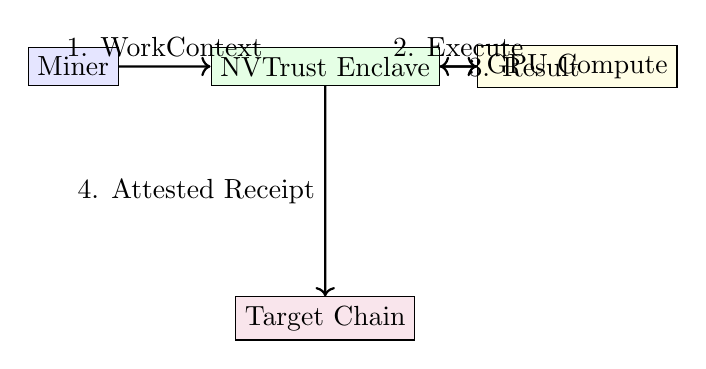
\begin{tikzpicture}[scale=0.8]
    \node[draw, rectangle, fill=blue!10] (miner) at (0,4) {Miner};
    \node[draw, rectangle, fill=green!10] (nvtrust) at (4,4) {NVTrust Enclave};
    \node[draw, rectangle, fill=yellow!10] (gpu) at (8,4) {GPU Compute};
    \node[draw, rectangle, fill=purple!10] (chain) at (4,0) {Target Chain};

    \draw[->, thick] (miner) -- node[above] {1. WorkContext} (nvtrust);
    \draw[->, thick] (nvtrust) -- node[above] {2. Execute} (gpu);
    \draw[->, thick] (gpu) -- node[right] {3. Result} (nvtrust);
    \draw[->, thick] (nvtrust) -- node[left] {4. Attested Receipt} (chain);
\end{tikzpicture}
\end{center}

\subsection{Attested Receipt}

The NVTrust enclave produces an \textbf{AttestedReceipt}:

\begin{lstlisting}[style=rust]
pub struct AttestedReceipt {
    pub context: WorkContext,         // Original commitment
    pub result_hash: [u8; 32],        // BLAKE3(output)
    pub work_metrics: WorkMetrics,    // FLOPs, tokens, time
    pub nvtrust_signature: Vec<u8>,   // GPU hardware signature
    pub spdm_evidence: SPDMEvidence,  // Firmware measurements
}

pub struct SPDMEvidence {
    pub version: u8,
    pub measurement_hash: [u8; 48],   // GPU firmware hash
    pub nonce: [u8; 32],              // Replay protection
    pub signature: Vec<u8>,           // SPDM signature
    pub certificate_chain: Vec<u8>,   // Chain to NVIDIA root
}
\end{lstlisting}

\subsection{Spent Set}

Each chain maintains a \textbf{SpentSet} to track minted work:

\begin{definition}[Work ID]
The unique identifier for a unit of work is:
\begin{equation}
\text{work\_id} = \text{BLAKE3}(\text{device\_id} \| \text{nonce} \| \text{chain\_id})
\end{equation}
\end{definition}

\begin{property}[Spent Set Invariant]
For all valid blocks $B$ and proofs $P \in B$:
\begin{equation}
\text{work\_id}(P) \notin \text{SpentSet}(B.\text{prev}) \land \text{work\_id}(P) \in \text{SpentSet}(B)
\end{equation}
\end{property}

\begin{algorithm}
\caption{CheckAndMarkSpent}
\begin{algorithmic}[1]
\Require AttestedReceipt $R$, SpentSet $S$
\Ensure Boolean (success), SpentSet (updated)
\State $\text{work\_id} \gets \text{BLAKE3}(R.\text{context}.\text{device\_id} \| R.\text{context}.\text{nonce} \| R.\text{context}.\text{chain\_id})$
\If{$\text{work\_id} \in S$}
    \State \Return (\textbf{false}, $S$) \Comment{Already minted}
\EndIf
\State $S' \gets S \cup \{\text{work\_id}\}$
\State \Return (\textbf{true}, $S'$)
\end{algorithmic}
\end{algorithm}

\subsection{Chain ID Validation}

Before processing any receipt, validators check chain binding:

\begin{lstlisting}[style=rust]
fn validate_chain_binding(
    receipt: &AttestedReceipt,
    expected_chain_id: u64,
) -> Result<(), MiningError> {
    if receipt.context.chain_id != expected_chain_id {
        return Err(MiningError::WrongChain {
            expected: expected_chain_id,
            got: receipt.context.chain_id,
        });
    }
    Ok(())
}
\end{lstlisting}

\subsection{Multi-Chain Mining}

The same GPU can mine for multiple chains, but requires \textbf{separate work} for each:

\begin{center}
\begin{tabular}{lccc}
\toprule
\textbf{GPU} & \textbf{Hanzo (36963)} & \textbf{Zoo (200200)} & \textbf{Lux (96369)} \\
\midrule
H100-001 & nonce: 0x1a... & nonce: 0x2b... & nonce: 0x3c... \\
H100-001 & Receipt A & Receipt B & Receipt C \\
H100-001 & \checkmark Valid & \checkmark Valid & \checkmark Valid \\
\bottomrule
\end{tabular}
\end{center}

\begin{lemma}[Cross-Chain Independence]
Receipts $R_A$ and $R_B$ with different chain IDs are independent:
\begin{equation}
\text{work\_id}(R_A) \neq \text{work\_id}(R_B) \iff R_A.\text{chain\_id} \neq R_B.\text{chain\_id}
\end{equation}
\end{lemma}

\subsection{Supported GPU Hardware}

\begin{center}
\begin{tabular}{lccc}
\toprule
\textbf{GPU Model} & \textbf{CC Support} & \textbf{Trust Score} & \textbf{Reward Multiplier} \\
\midrule
GB200 & Full NVTrust + TEE-I/O & 100 & 1.5x \\
B200 & Full NVTrust + TEE-I/O & 100 & 1.5x \\
B100 & Full NVTrust + TEE-I/O & 100 & 1.5x \\
H200 & Full NVTrust & 95 & 1.3x \\
H100 & Full NVTrust & 95 & 1.3x \\
RTX PRO 6000 & NVTrust & 85 & 1.1x \\
RTX 5090 & Software only & 60 & 0.8x \\
RTX 4090 & Software only & 60 & 0.8x \\
\bottomrule
\end{tabular}
\end{center}

\textbf{Key Invariant:} The same AI work cannot be minted on Hanzo, Lux, AND Zoo---only on the chain specified in the pre-committed WorkContext.chain\_id.

\section{Difficulty Adjustment}
\label{sec:difficulty}

\subsection{Overview}

Unlike Bitcoin's hash-based difficulty, PoAI uses a \textbf{compute-based difficulty} that adjusts based on network AI throughput. The goal is to maintain consistent block times while adapting to changes in total compute capacity.

\subsection{Difficulty Target}

\begin{definition}[Difficulty Target]
The difficulty target $D$ represents the minimum compute units required for a valid proof:
\begin{equation}
D = \text{base\_compute} \times 2^{\text{difficulty\_bits}}
\end{equation}
\end{definition}

A proof is valid only if:
\begin{equation}
W_{\text{proof}} \geq D_{\text{current}}
\end{equation}

\subsection{Adjustment Algorithm}

Difficulty adjusts every $N_{\text{adj}} = 2016$ blocks (similar to Bitcoin):

\begin{algorithm}
\caption{AdjustDifficulty}
\begin{algorithmic}[1]
\Require Previous difficulty $D_{\text{prev}}$, actual time $T_{\text{actual}}$, target time $T_{\text{target}}$
\Ensure New difficulty $D_{\text{new}}$
\State $\text{ratio} \gets T_{\text{actual}} / T_{\text{target}}$
\State $\text{ratio} \gets \max(0.25, \min(4.0, \text{ratio}))$ \Comment{Clamp to 4x range}
\State $D_{\text{new}} \gets D_{\text{prev}} / \text{ratio}$
\State \Return $D_{\text{new}}$
\end{algorithmic}
\end{algorithm}

\subsection{Per-Chain Difficulty}

Each chain maintains independent difficulty:

\begin{center}
\begin{tabular}{lcccc}
\toprule
\textbf{Chain} & \textbf{Target Block Time} & \textbf{Adjustment Window} & \textbf{Max Adjustment} \\
\midrule
Hanzo (36963) & 2 seconds & 2016 blocks & 4x \\
Zoo (200200) & 2 seconds & 2016 blocks & 4x \\
Lux (96369) & 2 seconds & 2016 blocks & 4x \\
\bottomrule
\end{tabular}
\end{center}

\subsection{Compute Unit Standardization}

Different AI workloads produce different compute metrics. We standardize to \textbf{AI Compute Units (ACU)}:

\begin{equation}
\text{ACU} = \alpha \times \text{tokens} + \beta \times \text{FLOPs} + \gamma \times \text{compute\_hours}
\end{equation}

where:
\begin{itemize}
    \item $\alpha = 10^{-3}$ (tokens to ACU)
    \item $\beta = 10^{-15}$ (FLOPs to ACU)
    \item $\gamma = 10^{6}$ (hours to ACU)
\end{itemize}

\subsection{GPU Tier Adjustment}

Higher-tier GPUs earn bonus difficulty credits:

\begin{equation}
D_{\text{effective}} = D_{\text{raw}} \times M_{\text{tier}}
\end{equation}

\begin{center}
\begin{tabular}{lcc}
\toprule
\textbf{GPU Tier} & \textbf{$M_{\text{tier}}$} & \textbf{Effective Difficulty} \\
\midrule
Sovereign (GB200, B200) & 1.5 & $D \times 1.5$ \\
DataCenter (H100, H200) & 1.3 & $D \times 1.3$ \\
Professional (RTX PRO) & 1.1 & $D \times 1.1$ \\
Consumer (RTX 4090/5090) & 0.8 & $D \times 0.8$ \\
\bottomrule
\end{tabular}
\end{center}

\subsection{Emergency Difficulty Adjustment}

If blocks are too slow (>10x target), emergency adjustment triggers:

\begin{lstlisting}[style=rust]
fn emergency_adjust(
    current_difficulty: u64,
    time_since_last_block: Duration,
    target_block_time: Duration,
) -> u64 {
    if time_since_last_block > target_block_time * 10 {
        // Emergency: reduce difficulty by 25%
        current_difficulty * 75 / 100
    } else {
        current_difficulty
    }
}
\end{lstlisting}

\subsection{Difficulty and Rewards}

Rewards scale inversely with difficulty:

\begin{equation}
R = R_{\text{base}} \times \frac{D_0}{D_{\text{current}}}
\end{equation}

This ensures:
\begin{itemize}
    \item High difficulty $\Rightarrow$ fewer proofs valid $\Rightarrow$ higher reward per proof
    \item Low difficulty $\Rightarrow$ more proofs valid $\Rightarrow$ lower reward per proof
\end{itemize}

\subsection{Economic Equilibrium}

\begin{theorem}[Mining Equilibrium]
In equilibrium, miners earn expected value equal to their electricity and hardware costs:
\begin{equation}
\mathbb{E}[\text{Revenue}] = \text{Cost}_{\text{electricity}} + \text{Cost}_{\text{depreciation}}
\end{equation}
Difficulty auto-adjusts to maintain this equilibrium as hashrate changes.
\end{theorem}

\section{Market Dynamics and Payment}
\label{sec:payments}

\subsection{Overview}

PoAI creates a two-sided market where:
\begin{itemize}
    \item \textbf{Miners} provide AI compute and earn AI tokens
    \item \textbf{Users} pay AI tokens for AI services (inference, training, etc.)
\end{itemize}

\subsection{Payment Flow}

\begin{center}
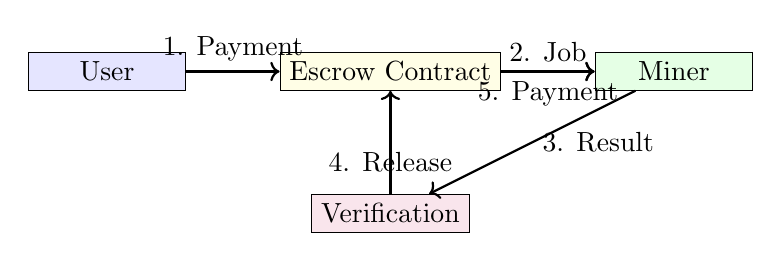
\begin{tikzpicture}[scale=0.9]
    \node[draw, rectangle, fill=blue!10, minimum width=2cm] (user) at (0,0) {User};
    \node[draw, rectangle, fill=yellow!10, minimum width=2cm] (escrow) at (4,0) {Escrow Contract};
    \node[draw, rectangle, fill=green!10, minimum width=2cm] (miner) at (8,0) {Miner};
    \node[draw, rectangle, fill=purple!10, minimum width=2cm] (verify) at (4,-2) {Verification};

    \draw[->, thick] (user) -- node[above] {1. Payment} (escrow);
    \draw[->, thick] (escrow) -- node[above] {2. Job} (miner);
    \draw[->, thick] (miner) -- node[right] {3. Result} (verify);
    \draw[->, thick] (verify) -- node[below] {4. Release} (escrow);
    \draw[->, thick] (escrow) -- node[below] {5. Payment} (miner);
\end{tikzpicture}
\end{center}

\subsection{Pricing Models}

Miners can offer multiple pricing models:

\begin{center}
\begin{tabular}{lll}
\toprule
\textbf{Model} & \textbf{Unit} & \textbf{Use Case} \\
\midrule
Per Token & AI/token & LLM inference \\
Per Inference & AI/request & Image generation \\
Per Minute & AI/minute & Real-time audio \\
Per FLOP & AI/TFLOP & Training \\
Hybrid & Mix & Custom workloads \\
\bottomrule
\end{tabular}
\end{center}

\subsection{Market-Driven Pricing}

Prices adjust based on supply and demand using \textbf{Hamiltonian market dynamics}:

\begin{definition}[Hamiltonian Market]
The market state is described by position $q$ (price) and momentum $p$ (order flow):
\begin{align}
\frac{dq}{dt} &= \frac{\partial H}{\partial p} = p \\
\frac{dp}{dt} &= -\frac{\partial H}{\partial q} - \gamma p + \xi(t)
\end{align}
where $H = \frac{p^2}{2} + V(q)$ is the Hamiltonian, $\gamma$ is damping, and $\xi(t)$ is noise.
\end{definition}

\subsubsection{Price Update Algorithm}

\begin{algorithm}
\caption{UpdateMarketPrice}
\begin{algorithmic}[1]
\Require Current price $P$, supply $S$, demand $D$, target utilization $U_{\text{target}}$
\Ensure New price $P'$
\State $U_{\text{current}} \gets D / S$ \Comment{Current utilization}
\State $\text{imbalance} \gets U_{\text{current}} - U_{\text{target}}$
\State $\text{adjustment} \gets \text{imbalance} \times \text{sensitivity}$
\State $\text{adjustment} \gets \text{adjustment} \times \text{damping}$ \Comment{Prevent oscillation}
\State $P' \gets P \times (1 + \text{adjustment})$
\State $P' \gets \max(P_{\text{min}}, \min(P_{\text{max}}, P'))$ \Comment{Bounds}
\State \Return $P'$
\end{algorithmic}
\end{algorithm}

\subsection{Escrow Contract}

Payments are held in escrow until work is verified:

\begin{lstlisting}[style=solidity]
contract ComputeEscrow {
    struct Request {
        address user;
        address miner;
        uint256 payment;
        bytes32 inputHash;
        bytes32 resultHash;
        uint256 deadline;
        RequestStatus status;
    }

    function createRequest(
        bytes32 modelId,
        bytes32 inputHash,
        uint256 maxPayment,
        uint256 deadline
    ) external returns (bytes32 requestId);

    function acceptRequest(bytes32 requestId) external;

    function submitResult(
        bytes32 requestId,
        bytes32 resultHash
    ) external;

    function verifyAndRelease(bytes32 requestId) external;

    function slashAndRefund(bytes32 requestId) external;
}
\end{lstlisting}

\subsection{Fee Structure}

\begin{center}
\begin{tabular}{lcc}
\toprule
\textbf{Fee Type} & \textbf{Rate} & \textbf{Recipient} \\
\midrule
Market Fee & 1\% & Protocol Treasury \\
Network Fee & Gas & Validators \\
Slashing & 10\% & User (refund) \\
\bottomrule
\end{tabular}
\end{center}

\subsection{Provider Registration}

Miners register as providers with stake:

\begin{lstlisting}[style=solidity]
function registerProvider(
    uint256 stake,           // Minimum 1000 AI
    bytes32 modelId,         // Supported model
    bytes32 gpuId,           // Hardware ID
    PricingModel memory pricing,
    uint256 maxConcurrent    // Max parallel jobs
) external;
\end{lstlisting}

\subsection{Slashing Conditions}

Providers are slashed (10\% of stake) for:
\begin{enumerate}
    \item \textbf{Invalid Result}: Output doesn't match input/model
    \item \textbf{Timeout}: No result by deadline
    \item \textbf{Attestation Failure}: NVTrust verification fails
\end{enumerate}

\subsection{Economic Incentives}

\begin{theorem}[Incentive Compatibility]
Under the escrow mechanism, honest behavior is a Nash equilibrium:
\begin{itemize}
    \item Miners: Providing valid compute maximizes expected profit
    \item Users: Paying for services maximizes utility
    \item Slashing cost exceeds fraud profit
\end{itemize}
\end{theorem}

\subsection{Per-Chain Fee Customization}

Each chain can set its own fee parameters:

\begin{center}
\begin{tabular}{lccc}
\toprule
\textbf{Parameter} & \textbf{Lux} & \textbf{Hanzo} & \textbf{Zoo} \\
\midrule
Base Price (AI/token) & 0.0001 & 0.0001 & 0.0001 \\
Market Fee & 1\% & 1\% & 2\% (research) \\
Min Provider Stake & 1000 AI & 1000 AI & 500 AI \\
Slashing Rate & 10\% & 10\% & 15\% \\
\bottomrule
\end{tabular}
\end{center}

This allows each chain's community to optimize for their specific use cases.

\section{Multi-Chain Mining with Teleport}
\label{sec:multi-chain}

\subsection{Overview}

PoAI enables seamless cross-chain operations via the \textbf{Teleport Protocol}. Miners can earn on any chain, and tokens can flow freely across the ecosystem.

\subsection{Supported Chains}

\begin{center}
\begin{tabular}{lccc}
\toprule
\textbf{Chain} & \textbf{Chain ID} & \textbf{Token} & \textbf{Role} \\
\midrule
Hanzo L1 & 36963 & AI (native) & Mining Origin \\
Hanzo EVM & 36963 & AI, ZOO & DeFi Hub \\
Zoo EVM & 200200 & AI, ZOO & Research Focus \\
Lux C-Chain & 96369 & AI, ZOO, LUX & General Purpose \\
\bottomrule
\end{tabular}
\end{center}

\subsection{Global Supply Dynamics}

\begin{property}[Expanding Global Cap]
The global AI supply cap increases only when new chains join:
\begin{equation}
S_{\text{global}} = n \times 10^9 \text{ AI}
\end{equation}
where $n$ is the number of active chains. This creates predictable scarcity while allowing ecosystem growth.
\end{property}

\subsection{Teleport Protocol}

\subsubsection{Architecture}

\begin{center}
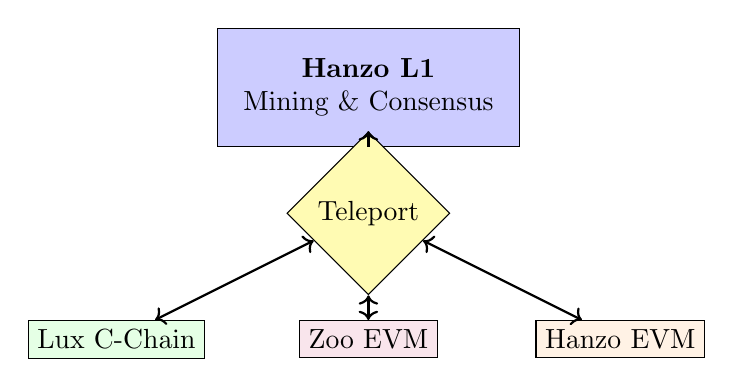
\begin{tikzpicture}[scale=0.8]
    \node[draw, rectangle, fill=blue!20, minimum width=3cm, minimum height=1.5cm] (hanzo) at (0,3) {
        \begin{tabular}{c}
        \textbf{Hanzo L1} \\
        Mining \& Consensus
        \end{tabular}
    };

    \node[draw, diamond, fill=yellow!30, minimum width=2cm] (teleport) at (0,1) {Teleport};

    \node[draw, rectangle, fill=green!10] (lux) at (-4,-1) {Lux C-Chain};
    \node[draw, rectangle, fill=purple!10] (zoo) at (0,-1) {Zoo EVM};
    \node[draw, rectangle, fill=orange!10] (hanzo_evm) at (4,-1) {Hanzo EVM};

    \draw[->, thick] (hanzo) -- (teleport);
    \draw[<->, thick] (teleport) -- (lux);
    \draw[<->, thick] (teleport) -- (zoo);
    \draw[<->, thick] (teleport) -- (hanzo_evm);
\end{tikzpicture}
\end{center}

\subsubsection{Transfer Flow}

\begin{enumerate}
    \item \textbf{Lock/Burn}: Source chain locks or burns tokens
    \item \textbf{MPC Validation}: Top 100 validators verify the transfer
    \item \textbf{Threshold Signature}: CGGMP20 produces collective signature
    \item \textbf{Mint/Release}: Destination chain mints or releases tokens
\end{enumerate}

\subsubsection{Transfer Message}

\begin{lstlisting}[style=rust]
pub struct TeleportTransfer {
    pub teleport_id: [u8; 32],       // Unique transfer ID
    pub source_chain: u64,           // Origin chain ID
    pub destination_chain: u64,      // Target chain ID
    pub sender: Vec<u8>,             // ML-DSA public key
    pub recipient: String,           // Destination address
    pub amount: u128,                // AI tokens (neurons)
    pub nonce: u64,                  // Replay protection
    pub timestamp: u64,              // Unix timestamp
    pub signature: Vec<u8>,          // ML-DSA signature
}
\end{lstlisting}

\subsection{Mining on Multiple Chains}

A single GPU can mine for all chains simultaneously by:

\begin{enumerate}
    \item Creating separate WorkContext for each chain
    \item Generating unique nonces per chain
    \item Submitting receipts to respective chains
\end{enumerate}

\begin{lstlisting}[style=rust]
// Mine for all three chains in parallel
let hanzo_ctx = WorkContext::for_chain(ChainId::Hanzo, &job);
let zoo_ctx = WorkContext::for_chain(ChainId::Zoo, &job);
let lux_ctx = WorkContext::for_chain(ChainId::Lux, &job);

// Execute and submit
let hanzo_receipt = execute_and_attest(hanzo_ctx).await?;
let zoo_receipt = execute_and_attest(zoo_ctx).await?;
let lux_receipt = execute_and_attest(lux_ctx).await?;

submit_to_chain(ChainId::Hanzo, hanzo_receipt).await?;
submit_to_chain(ChainId::Zoo, zoo_receipt).await?;
submit_to_chain(ChainId::Lux, lux_receipt).await?;
\end{lstlisting}

\textbf{Note}: Each submission requires \textit{separate work}---the same work cannot be submitted to multiple chains.

\subsection{Cross-Chain Reward Claiming}

Miners can claim rewards on any chain:

\begin{lstlisting}[style=solidity]
interface IRewardClaiming {
    // Claim reward mined on current chain
    function claimLocalReward(
        bytes calldata proof,
        bytes calldata signature
    ) external returns (uint256);

    // Claim reward mined on another chain via Teleport
    function claimCrossChainReward(
        bytes32 teleportId,
        bytes32[] calldata merkleProof
    ) external returns (uint256);
}
\end{lstlisting}

\subsection{Liquidity Pools}

Cross-chain liquidity enables efficient markets:

\begin{center}
\begin{tabular}{lcc}
\toprule
\textbf{Pool} & \textbf{Chain} & \textbf{Purpose} \\
\midrule
AI/ETH & Lux C-Chain & External liquidity \\
AI/ZOO & Zoo EVM & Governance pairing \\
AI/LUX & All & Native pairing \\
AI/USDC & All & Stable pairing \\
\bottomrule
\end{tabular}
\end{center}

\subsection{Chain-Specific Features}

\subsubsection{Lux C-Chain (96369)}
\begin{itemize}
    \item General-purpose EVM
    \item Highest liquidity
    \item Gateway to external ecosystems
\end{itemize}

\subsubsection{Hanzo EVM (36963)}
\begin{itemize}
    \item AI-focused applications
    \item Native mining origin
    \item Lowest latency for AI services
\end{itemize}

\subsubsection{Zoo EVM (200200)}
\begin{itemize}
    \item Research and DeSci focus
    \item Higher treasury allocation (2\%)
    \item Governance over research grants
\end{itemize}

\subsection{Adding New Chains}

New chains can join the ecosystem by:

\begin{enumerate}
    \item \textbf{Governance Proposal}: Submit proposal to add chain
    \item \textbf{Technical Integration}: Deploy Teleport contracts
    \item \textbf{Validator Opt-In}: MPC nodes monitor new chain
    \item \textbf{Supply Allocation}: 1B AI cap assigned to new chain
\end{enumerate}

\begin{equation}
S_{\text{global}}^{\text{new}} = S_{\text{global}}^{\text{old}} + 10^9
\end{equation}

\section{EVM Contracts}
\label{sec:evm-contracts}

\subsection{Overview}

PoAI deploys a suite of smart contracts on each EVM chain for mining reward management, token operations, and market functionality.

\subsection{Contract Architecture}

\begin{center}
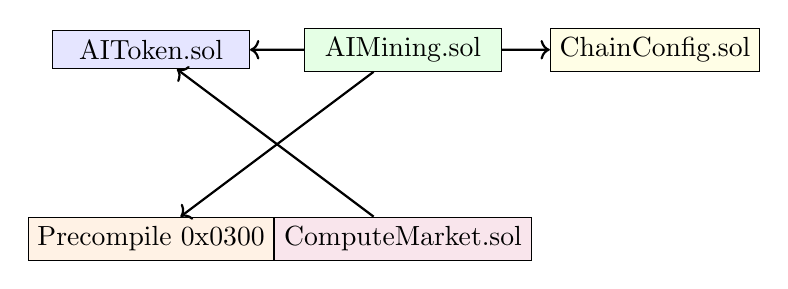
\begin{tikzpicture}[scale=0.8]
    \node[draw, rectangle, fill=blue!10, minimum width=2.5cm] (token) at (0,3) {AIToken.sol};
    \node[draw, rectangle, fill=green!10, minimum width=2.5cm] (mining) at (4,3) {AIMining.sol};
    \node[draw, rectangle, fill=yellow!10, minimum width=2.5cm] (config) at (8,3) {ChainConfig.sol};
    \node[draw, rectangle, fill=purple!10, minimum width=2.5cm] (market) at (4,0) {ComputeMarket.sol};
    \node[draw, rectangle, fill=orange!10, minimum width=2.5cm] (precompile) at (0,0) {Precompile 0x0300};

    \draw[->, thick] (mining) -- (token);
    \draw[->, thick] (mining) -- (config);
    \draw[->, thick] (market) -- (token);
    \draw[->, thick] (mining) -- (precompile);
\end{tikzpicture}
\end{center}

\subsection{AIToken.sol}

ERC20 token with mining-based minting:

\begin{lstlisting}[style=solidity]
contract AIToken is ERC20, AccessControl {
    uint256 public constant MAX_SUPPLY = 1_000_000_000 * 1e18;
    uint256 public constant HALVING_INTERVAL = 210_000;
    uint256 public constant INITIAL_REWARD = 50 * 1e18;
    uint256 public constant TREASURY_RATE = 200; // 2%

    uint256 public totalMinted;
    uint256 public genesisBlock;
    address public treasury;

    function mintReward(
        address miner,
        uint256 amount
    ) external onlyRole(MINER_ROLE) {
        require(totalMinted + amount <= MAX_SUPPLY, "Supply cap");

        uint256 treasuryAmount = amount * TREASURY_RATE / 10000;
        uint256 minerAmount = amount - treasuryAmount;

        _mint(miner, minerAmount);
        _mint(treasury, treasuryAmount);
        totalMinted += amount;

        emit RewardMinted(miner, minerAmount, currentEpoch());
    }

    function currentEpoch() public view returns (uint256) {
        return (block.number - genesisBlock) / HALVING_INTERVAL;
    }

    function currentReward() public view returns (uint256) {
        uint256 epoch = currentEpoch();
        return INITIAL_REWARD >> epoch; // Halving
    }
}
\end{lstlisting}

\subsection{AIMining.sol}

Core mining contract for proof submission:

\begin{lstlisting}[style=solidity]
contract AIMining {
    struct WorkProof {
        bytes32 sessionId;
        bytes32 nonce;
        bytes32 gpuId;
        bytes32 computeHash;
        uint256 timestamp;
        GPUTier tier;
        bytes signature;
    }

    mapping(bytes32 => bool) public spentProofs;
    IChainConfig public config;
    IAIToken public token;

    function submitProof(
        WorkProof calldata proof
    ) external returns (uint256 reward) {
        // 1. Compute work ID
        bytes32 workId = keccak256(abi.encodePacked(
            proof.gpuId,
            proof.nonce,
            block.chainid
        ));

        // 2. Check spent set
        require(!spentProofs[workId], "Already minted");

        // 3. Verify via precompile
        require(
            IAIMiningPrecompile(PRECOMPILE).verifyMLDSA(
                proof.gpuId,
                abi.encode(proof),
                proof.signature
            ),
            "Invalid signature"
        );

        // 4. Calculate reward
        reward = calculateReward(proof);

        // 5. Mark spent and mint
        spentProofs[workId] = true;
        token.mintReward(msg.sender, reward);

        emit ProofSubmitted(msg.sender, workId, reward);
    }

    function calculateReward(
        WorkProof calldata proof
    ) public view returns (uint256) {
        uint256 baseReward = token.currentReward();
        uint256 multiplier = config.getGPUMultiplier(proof.tier);
        return baseReward * multiplier / 10000;
    }
}
\end{lstlisting}

\subsection{ChainConfig.sol}

Per-chain configuration management:

\begin{lstlisting}[style=solidity]
contract ChainConfig {
    struct Config {
        uint256 baseReward;
        uint256 halvingInterval;
        uint256 difficultyTarget;
        uint256 treasuryRate;
        mapping(GPUTier => uint256) gpuMultipliers;
    }

    mapping(uint256 => Config) public chainConfigs;

    function initializeChain(
        uint256 chainId,
        uint256 baseReward,
        uint256 treasuryRate
    ) external onlyAdmin {
        Config storage cfg = chainConfigs[chainId];
        cfg.baseReward = baseReward;
        cfg.halvingInterval = 210_000;
        cfg.treasuryRate = treasuryRate;

        // Default GPU multipliers
        cfg.gpuMultipliers[GPUTier.Consumer] = 8000;     // 0.8x
        cfg.gpuMultipliers[GPUTier.Professional] = 11000; // 1.1x
        cfg.gpuMultipliers[GPUTier.DataCenter] = 13000;   // 1.3x
        cfg.gpuMultipliers[GPUTier.Sovereign] = 15000;    // 1.5x
    }

    function getGPUMultiplier(
        GPUTier tier
    ) external view returns (uint256) {
        return chainConfigs[block.chainid].gpuMultipliers[tier];
    }
}
\end{lstlisting}

\subsection{ComputeMarket.sol}

Decentralized AI service marketplace:

\begin{lstlisting}[style=solidity]
contract ComputeMarket {
    struct Provider {
        uint256 stake;
        bytes32 modelId;
        bytes32 gpuId;
        PricingModel pricing;
        uint256 activeRequests;
        uint256 maxConcurrent;
        uint256 reputation;
    }

    struct Request {
        address user;
        address provider;
        bytes32 modelId;
        bytes32 inputHash;
        bytes32 resultHash;
        uint256 payment;
        uint256 deadline;
        RequestStatus status;
    }

    mapping(address => Provider) public providers;
    mapping(bytes32 => Request) public requests;

    function createRequest(
        bytes32 modelId,
        bytes32 inputHash,
        uint256 maxPayment,
        uint256 duration
    ) external returns (bytes32 requestId) {
        // Transfer payment to escrow
        token.transferFrom(msg.sender, address(this), maxPayment);

        requestId = keccak256(abi.encodePacked(
            msg.sender,
            modelId,
            block.timestamp
        ));

        requests[requestId] = Request({
            user: msg.sender,
            provider: address(0),
            modelId: modelId,
            inputHash: inputHash,
            resultHash: bytes32(0),
            payment: maxPayment,
            deadline: block.timestamp + duration,
            status: RequestStatus.Open
        });
    }

    function submitResult(
        bytes32 requestId,
        bytes32 resultHash
    ) external {
        Request storage req = requests[requestId];
        require(req.provider == msg.sender, "Not provider");
        require(req.status == RequestStatus.Accepted, "Not accepted");

        req.resultHash = resultHash;
        req.status = RequestStatus.Completed;

        // Release payment minus market fee
        uint256 fee = req.payment * MARKET_FEE / 10000;
        token.transfer(msg.sender, req.payment - fee);
        token.transfer(treasury, fee);
    }
}
\end{lstlisting}

\subsection{Precompile Interface}

High-performance native operations at address \texttt{0x0300}:

\begin{lstlisting}[style=solidity]
interface IAIMiningPrecompile {
    /// @notice Verify ML-DSA quantum-safe signature
    /// @param pubkey ML-DSA public key (1952 bytes for Level 3)
    /// @param message Message that was signed
    /// @param signature ML-DSA signature
    /// @return valid True if signature is valid
    function verifyMLDSA(
        bytes calldata pubkey,
        bytes calldata message,
        bytes calldata signature
    ) external view returns (bool valid);

    /// @notice Calculate reward for work proof
    /// @param workProof Encoded work proof
    /// @param chainId Target chain ID
    /// @return reward Calculated reward in neurons
    function calculateReward(
        bytes calldata workProof,
        uint64 chainId
    ) external view returns (uint256 reward);

    /// @notice Verify NVTrust GPU attestation
    /// @param receipt Attested receipt from NVTrust
    /// @param signature NVTrust signature
    /// @return valid True if attestation is valid
    function verifyNVTrust(
        bytes calldata receipt,
        bytes calldata signature
    ) external view returns (bool valid);

    /// @notice Check if work ID is in spent set
    /// @param workId Work identifier
    /// @return spent True if already minted
    function isSpent(bytes32 workId) external view returns (bool spent);

    /// @notice Compute work ID from components
    /// @param deviceId GPU device ID
    /// @param nonce Unique nonce
    /// @param chainId Target chain ID
    /// @return workId Computed work identifier
    function computeWorkId(
        bytes32 deviceId,
        bytes32 nonce,
        uint64 chainId
    ) external pure returns (bytes32 workId);
}
\end{lstlisting}

\subsection{Gas Costs}

\begin{center}
\begin{tabular}{lcc}
\toprule
\textbf{Operation} & \textbf{Precompile} & \textbf{Pure Solidity} \\
\midrule
verifyMLDSA & 3,000 gas & 500,000+ gas \\
calculateReward & 1,000 gas & 10,000 gas \\
verifyNVTrust & 5,000 gas & 1,000,000+ gas \\
isSpent & 100 gas & 2,100 gas (SLOAD) \\
computeWorkId & 50 gas & 500 gas \\
\bottomrule
\end{tabular}
\end{center}

\subsection{Deployment Addresses}

\begin{center}
\begin{tabular}{llc}
\toprule
\textbf{Contract} & \textbf{Address} & \textbf{All Chains} \\
\midrule
AIToken & 0xAI00...0001 & \checkmark \\
AIMining & 0xAI00...0002 & \checkmark \\
ChainConfig & 0xAI00...0003 & \checkmark \\
ComputeMarket & 0xAI00...0004 & \checkmark \\
Precompile & 0x0300 & \checkmark \\
\bottomrule
\end{tabular}
\end{center}

\section{Security Analysis}
\label{sec:security}

\subsection{Threat Model}

We consider adversaries with the following capabilities:

\begin{enumerate}
    \item \textbf{Malicious Miners}: Control GPU hardware, attempt double-spend
    \item \textbf{Network Attackers}: Observe and manipulate network traffic
    \item \textbf{Quantum Adversaries}: Future quantum computers attacking signatures
    \item \textbf{Colluding Validators}: Up to $f < n/3$ Byzantine validators
\end{enumerate}

\subsection{Quantum Safety}

\subsubsection{ML-DSA Signatures}

All mining signatures use ML-DSA (FIPS 204), providing NIST Level 3 security:

\begin{center}
\begin{tabular}{lccc}
\toprule
\textbf{Algorithm} & \textbf{Classical} & \textbf{Quantum} & \textbf{Key Size} \\
\midrule
ECDSA (current) & 128-bit & $\sim$64-bit & 33 bytes \\
ML-DSA-65 & 192-bit & 128-bit & 1,952 bytes \\
\bottomrule
\end{tabular}
\end{center}

\begin{theorem}[Quantum Resistance]
Under the Module-LWE hardness assumption, ML-DSA signatures are existentially unforgeable under chosen-message attack with quantum adversaries.
\end{theorem}

\subsubsection{Quantum Timeline}

\begin{center}
\begin{tabular}{lcc}
\toprule
\textbf{Year} & \textbf{Threat Level} & \textbf{Mitigation} \\
\midrule
2024--2026 & Low & ML-DSA optional \\
2026--2028 & Medium & ML-DSA default \\
2030+ & High & ECDSA deprecated \\
\bottomrule
\end{tabular}
\end{center}

\subsection{Double-Spend Prevention}

\subsubsection{Spent Set Security}

\begin{lemma}[Spent Set Collision Resistance]
The probability of two distinct work units having the same work ID is:
\begin{equation}
P(\text{collision}) \leq \frac{q^2}{2^{257}} \approx 0
\end{equation}
where $q$ is the number of work units and we use 256-bit BLAKE3.
\end{lemma}

\subsubsection{Chain Binding Security}

\begin{theorem}[Chain Binding Unforgeability]
An adversary cannot produce a valid receipt for chain $C_2$ from work performed for chain $C_1$:
\begin{equation}
\text{Adv}_{\text{forge}}^{\text{chain-bind}}(\mathcal{A}) \leq \text{Adv}_{\text{forge}}^{\text{NVTrust}}(\mathcal{A}) + \text{negl}(\lambda)
\end{equation}
\end{theorem}

\begin{proof}
Chain ID is included in the NVTrust-signed receipt. Modifying the chain ID invalidates the signature. Creating a new valid signature requires breaking NVTrust attestation security.
\end{proof}

\subsection{NVTrust Security}

\subsubsection{Trust Assumptions}

\begin{enumerate}
    \item NVIDIA root CA is trusted and not compromised
    \item GPU firmware is correctly implemented
    \item SPDM protocol is secure against replay and modification
    \item Hardware attestation keys are protected by GPU TEE
\end{enumerate}

\subsubsection{Attestation Chain}

\begin{center}
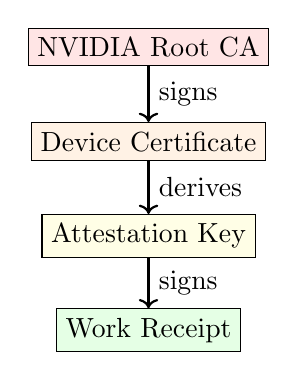
\begin{tikzpicture}[scale=0.8]
    \node[draw, rectangle, fill=red!10] (nvidia) at (0,3) {NVIDIA Root CA};
    \node[draw, rectangle, fill=orange!10] (device) at (0,1.5) {Device Certificate};
    \node[draw, rectangle, fill=yellow!10] (att) at (0,0) {Attestation Key};
    \node[draw, rectangle, fill=green!10] (receipt) at (0,-1.5) {Work Receipt};

    \draw[->, thick] (nvidia) -- node[right] {signs} (device);
    \draw[->, thick] (device) -- node[right] {derives} (att);
    \draw[->, thick] (att) -- node[right] {signs} (receipt);
\end{tikzpicture}
\end{center}

\subsection{Consensus Security}

\subsubsection{Quasar BFT Guarantees}

With $n$ validators and $f < n/3$ Byzantine:

\begin{property}[Safety]
No two honest validators finalize conflicting blocks:
\begin{equation}
\forall v_1, v_2 \in \text{Honest}: \text{finalized}(v_1) \cap \text{finalized}(v_2) \text{ is consistent}
\end{equation}
\end{property}

\begin{property}[Liveness]
If $\geq 2n/3$ validators are honest and network is synchronous, blocks finalize:
\begin{equation}
\forall \text{tx}: \exists t: \text{finalized}(\text{tx}) \text{ by time } t
\end{equation}
\end{property}

\subsection{Teleport Security}

\subsubsection{MPC Security}

Teleport uses CGGMP20 threshold ECDSA with $t$-of-$n$ security:

\begin{theorem}[Threshold Security]
The combined private key is never reconstructed. At least $t$ parties must collude to sign.
\end{theorem}

\subsubsection{Replay Protection}

Each transfer has a unique ID:
\begin{equation}
\text{teleport\_id} = \text{BLAKE3}(\text{source} \| \text{dest} \| \text{sender} \| \text{amount} \| \text{nonce})
\end{equation}

\subsection{Economic Security}

\subsubsection{Mining Attacks}

\begin{center}
\begin{tabular}{lcc}
\toprule
\textbf{Attack} & \textbf{Cost} & \textbf{Mitigation} \\
\midrule
Double-spend & NVTrust break & Hardware attestation \\
Selfish mining & Opportunity cost & Instant finality \\
Empty blocks & No reward & Work requirement \\
\bottomrule
\end{tabular}
\end{center}

\subsubsection{Slashing Conditions}

Misbehaving providers lose stake:

\begin{center}
\begin{tabular}{lc}
\toprule
\textbf{Violation} & \textbf{Penalty} \\
\midrule
Invalid compute result & 10\% stake \\
Timeout / no response & 10\% stake \\
Attestation fraud & 100\% stake \\
Double-sign & 100\% stake \\
\bottomrule
\end{tabular}
\end{center}

\subsection{Key Zeroization}

All secret keys are zeroized on drop:

\begin{lstlisting}[style=rust]
#[derive(Zeroize, ZeroizeOnDrop)]
pub struct SecretKey(Vec<u8>);

impl Drop for SecretKey {
    fn drop(&mut self) {
        self.0.zeroize();
    }
}
\end{lstlisting}

\subsection{Audit Status}

\begin{center}
\begin{tabular}{lcc}
\toprule
\textbf{Component} & \textbf{Auditor} & \textbf{Status} \\
\midrule
Smart Contracts & TBD & Pending \\
ML-DSA Implementation & TBD & Pending \\
NVTrust Integration & TBD & Pending \\
Teleport Protocol & TBD & Pending \\
\bottomrule
\end{tabular}
\end{center}

\section{Conclusion}
\label{sec:conclusion}

\subsection{Summary}

Proof of AI (PoAI) establishes an open protocol for decentralized AI mining with the following key properties:

\begin{enumerate}
    \item \textbf{Open Participation}: Anyone with GPU compute can mine AI tokens
    \item \textbf{Useful Work}: Rewards actual AI computation, not wasteful hashing
    \item \textbf{Bitcoin Economics}: 1B supply cap per chain, halving schedule
    \item \textbf{Quantum Safety}: ML-DSA signatures protect long-term value
    \item \textbf{Multi-Chain}: Seamless operation across Hanzo, Zoo, and Lux
    \item \textbf{Double-Spend Proof}: NVTrust chain-binding prevents fraud
    \item \textbf{Market Dynamics}: Supply/demand pricing for AI services
    \item \textbf{Future Privacy}: Upgrade path to shielded mining via ZK proofs
\end{enumerate}

\subsection{Ecosystem Benefits}

\subsubsection{For Miners}
\begin{itemize}
    \item Monetize idle GPU capacity
    \item Earn from multiple chains simultaneously
    \item Higher rewards for premium hardware
    \item Quantum-safe earnings protection
\end{itemize}

\subsubsection{For Users}
\begin{itemize}
    \item Access to decentralized AI compute
    \item Market-driven competitive pricing
    \item Cross-chain token portability
    \item Trustless escrow payments
\end{itemize}

\subsubsection{For Developers}
\begin{itemize}
    \item Standard interfaces across all chains
    \item Precompiles for efficient operations
    \item Open-source reference implementations
    \item Comprehensive documentation
\end{itemize}

\subsection{Comparison with Alternatives}

\begin{center}
\begin{tabular}{lccccc}
\toprule
\textbf{Property} & \textbf{PoAI} & \textbf{Bitcoin} & \textbf{PoS} & \textbf{Render} & \textbf{Akash} \\
\midrule
Useful work & \checkmark & & & \checkmark & \checkmark \\
Fixed supply & \checkmark & \checkmark & & & \\
Quantum-safe & \checkmark & & & & \\
Multi-chain & \checkmark & & & & \\
Hardware TEE & \checkmark & & & & \\
Instant finality & \checkmark & & \checkmark & & \\
\bottomrule
\end{tabular}
\end{center}

\subsection{Roadmap}

\begin{center}
\begin{tabular}{lcl}
\toprule
\textbf{Version} & \textbf{Target} & \textbf{Features} \\
\midrule
v1.0 & Q1 2025 & Public mining with NVTrust \\
v1.1 & Q2 2025 & Compute marketplace launch \\
v1.2 & Q3 2025 & Additional GPU support \\
v2.0 & Q4 2025 & Optional shielded mining (ZK) \\
v2.1 & Q1 2026 & Cross-chain atomic swaps \\
v3.0 & Q2 2026 & Default shielded mining \\
\bottomrule
\end{tabular}
\end{center}

\subsection{Future Work}

\subsubsection{Near-Term}
\begin{enumerate}
    \item Complete NVTrust SDK integration
    \item Security audits of all contracts
    \item Testnet deployment and stress testing
    \item Developer documentation and tutorials
\end{enumerate}

\subsubsection{Medium-Term}
\begin{enumerate}
    \item ZK circuit implementation for shielded mining
    \item Additional chain integrations
    \item Mobile wallet support
    \item Hardware wallet integration
\end{enumerate}

\subsubsection{Long-Term}
\begin{enumerate}
    \item Fully homomorphic compute verification
    \item Decentralized model training coordination
    \item AI governance via token voting
    \item Integration with external AI ecosystems
\end{enumerate}

\subsection{Open Source}

All PoAI implementations are open source:

\begin{center}
\begin{tabular}{ll}
\toprule
\textbf{Component} & \textbf{Repository} \\
\midrule
Protocol Specification & \texttt{github.com/luxfi/ai} \\
Smart Contracts & \texttt{github.com/luxfi/standard} \\
Mining Client & \texttt{github.com/hanzoai/node} \\
Precompiles & \texttt{github.com/luxfi/precompiles} \\
Documentation & \texttt{github.com/luxfi/ai/docs} \\
\bottomrule
\end{tabular}
\end{center}

\subsection{Acknowledgments}

The PoAI protocol draws on the work of many researchers and developers:

\begin{itemize}
    \item Satoshi Nakamoto for Bitcoin's elegant economic design
    \item NVIDIA for NVTrust confidential computing
    \item NIST for ML-DSA standardization
    \item The Lux, Hanzo, and Zoo communities
\end{itemize}

\subsection{Closing Remarks}

Proof of AI represents a fundamental shift in how we think about AI compute. By combining Bitcoin's elegant economic model with useful AI work, quantum-safe cryptography, and multi-chain interoperability, PoAI creates an open foundation for the AI economy.

\textit{``The future of AI should be open, decentralized, and owned by everyone who contributes.''}

\vspace{1em}
\begin{center}
\textbf{Build the future. Mine AI.}
\end{center}

\section{Shielded Mining via Zero-Knowledge Proofs}
\label{sec:zkproofs}

\subsection{Overview}

While public mining (Section~\ref{sec:proof-of-ai}) establishes a transparent economy, many miners require privacy for competitive or regulatory reasons. \textbf{Shielded Mining} integrates with the Lux Z-Chain to enable:

\begin{enumerate}
    \item \textbf{Hidden Miner Identity}: Device IDs and public keys masked via nullifiers
    \item \textbf{Hidden Workloads}: Model, input, and output data remain private
    \item \textbf{Verifiable Compute}: ZK proofs attest to valid AI work without revealing details
    \item \textbf{Selective Disclosure}: Gradual reveal for auditing when required
\end{enumerate}

\subsection{Z-Chain Integration}

The Lux Z-Chain provides the cryptographic infrastructure for shielded mining. Work proofs submitted to Z-Chain replace public data with ZK commitments.

\begin{definition}[Shielded Work Proof]
A shielded work proof $\pi$ consists of:
\begin{align}
\pi = (\text{commitment}, \text{nullifier}, \text{zkproof}, \text{timestamp})
\end{align}
where:
\begin{itemize}
    \item $\text{commitment} = \text{Commit}(\text{device\_id}, \text{work\_data}, r)$ for random $r$
    \item $\text{nullifier}$ prevents double-spend without revealing identity
    \item $\text{zkproof}$ attests to valid AI work
    \item $\text{timestamp}$ binds the proof to a time window
\end{itemize}
\end{definition}

\subsubsection{Commitment Scheme}

We use Pedersen commitments over the BLS12-381 curve:

\begin{equation}
\text{Commit}(m, r) = m \cdot G + r \cdot H
\end{equation}

where $G$ and $H$ are independent generators. This provides:
\begin{itemize}
    \item \textbf{Hiding}: Given $\text{Commit}(m, r)$, $m$ is computationally hidden
    \item \textbf{Binding}: Cannot find $(m', r')$ such that $\text{Commit}(m, r) = \text{Commit}(m', r')$
\end{itemize}

\subsection{Nullifier Scheme}

The nullifier scheme prevents double-spend while hiding miner identity.

\begin{definition}[Nullifier]
For a miner with secret key $\text{sk}$ and work identifier $\text{work\_id}$:
\begin{equation}
\text{nullifier} = \mathcal{H}(\text{sk} \| \text{work\_id})
\end{equation}
where $\mathcal{H}$ is a collision-resistant hash function (BLAKE3).
\end{definition}

\begin{property}[Double-Spend Prevention]
The spent set $\mathcal{S}$ stores nullifiers, not work IDs. A proof $\pi$ is rejected if:
\begin{equation}
\pi.\text{nullifier} \in \mathcal{S}
\end{equation}
This prevents double-spend without revealing which work was performed or by whom.
\end{property}

\subsubsection{Nullifier Properties}

\begin{enumerate}
    \item \textbf{Uniqueness}: Each (miner, work) pair produces a unique nullifier
    \item \textbf{Unlinkability}: Different nullifiers from the same miner cannot be linked
    \item \textbf{Non-forgery}: Cannot produce valid nullifier without knowing $\text{sk}$
\end{enumerate}

\begin{lemma}[Nullifier Security]
Under the collision resistance of $\mathcal{H}$:
\begin{enumerate}
    \item An adversary cannot find $(\text{sk}', \text{work\_id}')$ producing the same nullifier as honest $(\text{sk}, \text{work\_id})$
    \item Given nullifiers $n_1, n_2$ from the same miner, distinguishing them from random requires breaking the PRF property of $\mathcal{H}$
\end{enumerate}
\end{lemma}

\subsection{ZK Circuit Design}

The ZK circuit proves: ``I performed valid AI work for chain $C$ with nonce $N$'' without revealing device ID, model, or input/output data.

\subsubsection{Circuit Statement}

\begin{definition}[ZK Statement]
Public inputs:
\begin{align}
\mathbf{x} = (\text{chain\_id}, \text{commitment}, \text{nullifier}, \text{work\_type}, \text{compute\_units}, \text{timestamp})
\end{align}
Private witness:
\begin{align}
\mathbf{w} = (\text{sk}, \text{device\_id}, \text{nonce}, \text{model\_hash}, \text{input\_hash}, \text{output\_hash}, r)
\end{align}
\end{definition}

The circuit enforces:

\begin{equation}
\mathcal{R}(\mathbf{x}, \mathbf{w}) = 1 \iff
\begin{cases}
\text{commitment} = \text{Commit}((\text{device\_id}, \text{model\_hash}, \text{input\_hash}, \text{output\_hash}), r) \\
\text{nullifier} = \mathcal{H}(\text{sk} \| \text{device\_id} \| \text{nonce} \| \text{chain\_id}) \\
\text{ValidWork}(\text{work\_type}, \text{compute\_units}, \text{model\_hash}) = 1 \\
\text{NVTrustVerify}(\text{device\_id}, \text{model\_hash}, \text{input\_hash}, \text{output\_hash}) = 1
\end{cases}
\end{equation}

\subsubsection{Circuit Pseudocode}

\begin{algorithm}
\caption{ShieldedWorkCircuit}
\begin{algorithmic}[1]
\Require Public: $(\text{chain\_id}, \text{commitment}, \text{nullifier}, \text{work\_type}, \text{compute\_units}, \text{timestamp})$
\Require Private: $(\text{sk}, \text{device\_id}, \text{nonce}, \text{model\_hash}, \text{input\_hash}, \text{output\_hash}, r)$
\Ensure Boolean: circuit satisfiability

\State \Comment{1. Verify commitment opening}
\State $\text{data} \gets \text{Pack}(\text{device\_id}, \text{model\_hash}, \text{input\_hash}, \text{output\_hash})$
\State \textbf{assert} $\text{commitment} = \text{PedersenCommit}(\text{data}, r)$

\State \Comment{2. Verify nullifier derivation}
\State $\text{preimage} \gets \text{sk} \| \text{device\_id} \| \text{nonce} \| \text{chain\_id}$
\State \textbf{assert} $\text{nullifier} = \text{BLAKE3}(\text{preimage})$

\State \Comment{3. Verify work validity}
\If{$\text{work\_type} = \text{INFERENCE}$}
    \State \textbf{assert} $\text{compute\_units} \geq \text{MIN\_INFERENCE\_UNITS}$
    \State \textbf{assert} $\text{model\_hash} \in \text{APPROVED\_MODELS}$
\ElsIf{$\text{work\_type} = \text{TRAINING}$}
    \State \textbf{assert} $\text{compute\_units} \geq \text{MIN\_TRAINING\_FLOPS}$
\ElsIf{$\text{work\_type} = \text{RESEARCH}$}
    \State \textbf{assert} $\text{compute\_units} \geq \text{MIN\_RESEARCH\_HOURS}$
\EndIf

\State \Comment{4. Verify NVTrust attestation (in-circuit)}
\State $\text{attestation} \gets \text{NVTrustAttestation}(\text{device\_id})$
\State \textbf{assert} $\text{VerifySignature}(\text{attestation}, \text{NVIDIA\_ROOT\_PK})$
\State \textbf{assert} $\text{attestation.device\_id} = \text{device\_id}$

\State \Comment{5. Verify timestamp freshness (relative check)}
\State \textbf{assert} $\text{timestamp} > 0$

\State \Return \textbf{true}
\end{algorithmic}
\end{algorithm}

\subsubsection{Proving System Selection}

\begin{center}
\begin{tabular}{lccc}
\toprule
\textbf{System} & \textbf{Proof Size} & \textbf{Verify Time} & \textbf{Setup} \\
\midrule
Groth16 & 128 bytes & 3ms & Trusted \\
PLONK & 400 bytes & 8ms & Universal \\
Halo2 & 600 bytes & 12ms & None \\
\bottomrule
\end{tabular}
\end{center}

\textbf{Recommendation}: Use \textbf{Groth16} for production (smallest proofs, fastest verification) with a trusted setup ceremony. Use \textbf{PLONK} for development and chains requiring universal setup.

\subsubsection{Circuit Constraints}

The circuit requires approximately:
\begin{itemize}
    \item \textbf{Pedersen commitment}: $\sim$1,500 constraints
    \item \textbf{BLAKE3 hash}: $\sim$25,000 constraints per invocation
    \item \textbf{NVTrust signature verification}: $\sim$200,000 constraints (BLS)
    \item \textbf{Range checks and logic}: $\sim$5,000 constraints
\end{itemize}

Total: $\sim$250,000 constraints (Groth16 proving time: $\sim$5 seconds on modern CPU).

\subsection{Privacy Levels}

Shielded mining supports multiple privacy levels, allowing miners to choose their disclosure preference.

\begin{definition}[Privacy Levels]
\begin{align}
\text{Level 0 (Public)} &: \text{All data public} \\
\text{Level 1 (Identity)} &: \text{Miner identity hidden} \\
\text{Level 2 (Workload)} &: \text{Model and I/O hidden} \\
\text{Level 3 (Full)} &: \text{All data in ZK}
\end{align}
\end{definition}

\begin{center}
\begin{tabular}{lcccc}
\toprule
\textbf{Data Field} & \textbf{Level 0} & \textbf{Level 1} & \textbf{Level 2} & \textbf{Level 3} \\
\midrule
Miner pubkey & Public & Hidden & Hidden & Hidden \\
Device ID & Public & Hidden & Hidden & Hidden \\
Chain ID & Public & Public & Public & Hidden$^*$ \\
Model hash & Public & Public & Hidden & Hidden \\
Input hash & Public & Public & Hidden & Hidden \\
Output hash & Public & Public & Hidden & Hidden \\
Compute units & Public & Public & Public & Hidden$^*$ \\
Work type & Public & Public & Public & Hidden$^*$ \\
\bottomrule
\end{tabular}
\end{center}

$^*$Level 3 hides these in ZK but proves they meet minimum thresholds.

\subsubsection{Level 1: Hidden Miner Identity}

Only the nullifier is exposed; device ID and public key are hidden.

\begin{lstlisting}[style=rust]
pub struct Level1ShieldedProof {
    // Public
    pub nullifier: [u8; 32],
    pub chain_id: u64,
    pub model_hash: [u8; 32],
    pub input_hash: [u8; 32],
    pub output_hash: [u8; 32],
    pub compute_units: u64,
    pub timestamp: u64,

    // ZK proof that hidden identity is valid
    pub zk_proof: Vec<u8>,
}
\end{lstlisting}

\subsubsection{Level 2: Hidden Workload}

Model and I/O data are hidden; only compute units and work type are public.

\begin{lstlisting}[style=rust]
pub struct Level2ShieldedProof {
    // Public
    pub nullifier: [u8; 32],
    pub chain_id: u64,
    pub work_type: WorkType,
    pub compute_units: u64,
    pub timestamp: u64,

    // Commitments to hidden data
    pub model_commitment: [u8; 32],
    pub io_commitment: [u8; 32],

    // ZK proof
    pub zk_proof: Vec<u8>,
}
\end{lstlisting}

\subsubsection{Level 3: Fully Shielded}

All data hidden; ZK proof attests to minimum thresholds.

\begin{lstlisting}[style=rust]
pub struct Level3ShieldedProof {
    // Only commitment and nullifier exposed
    pub commitment: [u8; 32],
    pub nullifier: [u8; 32],
    pub timestamp: u64,

    // ZK proof attesting to:
    // - Valid chain binding
    // - compute_units >= MIN_THRESHOLD
    // - work_type in {INFERENCE, TRAINING, RESEARCH}
    // - Valid NVTrust attestation
    pub zk_proof: Vec<u8>,
}
\end{lstlisting}

\subsection{Selective Disclosure}

Miners may need to reveal data for auditing, dispute resolution, or regulatory compliance. The protocol supports gradual disclosure.

\begin{definition}[Opening]
An opening $o$ for commitment $c = \text{Commit}(m, r)$ is the tuple $(m, r)$. Given $o$, anyone can verify:
\begin{equation}
c \stackrel{?}{=} \text{Commit}(m, r)
\end{equation}
\end{definition}

\subsubsection{Disclosure Levels}

\begin{enumerate}
    \item \textbf{Identity Disclosure}: Reveal $(device\_id, \text{sk\_commitment})$ to prove ownership
    \item \textbf{Work Disclosure}: Reveal $(model\_hash, input\_hash, output\_hash)$ to prove work details
    \item \textbf{Full Disclosure}: Reveal all witness data, converting to Level 0 proof
\end{enumerate}

\begin{algorithm}
\caption{SelectiveDisclosure}
\begin{algorithmic}[1]
\Require ShieldedProof $\pi$, DisclosureRequest $D$, MinerSecret $\text{sk}$
\Ensure DisclosureProof $\delta$
\If{$D.\text{level} = \text{IDENTITY}$}
    \State $\delta \gets (device\_id, \text{Commit}(\text{sk}, r'))$
    \State $\delta.\text{proof} \gets \text{ProveKnowledge}(\text{sk}, r')$
\ElsIf{$D.\text{level} = \text{WORK}$}
    \State $\delta \gets (model\_hash, input\_hash, output\_hash, r)$
    \State \textbf{verify} $\pi.\text{commitment} = \text{Commit}(\delta, r)$
\ElsIf{$D.\text{level} = \text{FULL}$}
    \State $\delta \gets (\text{sk}, device\_id, nonce, model\_hash, input\_hash, output\_hash, r)$
\EndIf
\State \Return $\delta$
\end{algorithmic}
\end{algorithm}

\subsection{Upgrade Path}

The protocol evolves from fully public to default shielded over multiple versions.

\begin{definition}[Version Timeline]
\begin{align}
\text{v1.0} &: \text{Public mining with NVTrust (current)} \\
\text{v2.0} &: \text{Optional shielded mining via Z-Chain} \\
\text{v3.0} &: \text{Default shielded with public opt-in}
\end{align}
\end{definition}

\subsubsection{v1.0: Public Mining (Current)}

All mining is public as described in Section~\ref{sec:proof-of-ai}. This establishes:
\begin{itemize}
    \item Baseline security model with NVTrust
    \item Economic equilibrium and difficulty adjustment
    \item Infrastructure for reward distribution
\end{itemize}

\subsubsection{v2.0: Optional Shielded Mining}

Miners may choose shielded mode by submitting proofs to Z-Chain.

\begin{lstlisting}[style=rust]
pub enum MiningMode {
    Public,           // Standard AIWorkProof
    Shielded(Level),  // Level1/2/3 ShieldedProof
}

pub struct MiningConfig {
    pub mode: MiningMode,
    pub chain_id: u64,
    pub zk_prover: Option<ProverConfig>,
}
\end{lstlisting}

\textbf{Transition Rules}:
\begin{enumerate}
    \item Shielded proofs receive \textbf{same rewards} as public proofs
    \item Spent sets are \textbf{unified}: nullifiers and work IDs share the same set
    \item Shielded-to-public \textbf{conversion} allowed via full disclosure
\end{enumerate}

\subsubsection{v3.0: Default Shielded}

Privacy becomes the default; public mining requires explicit opt-in.

\begin{itemize}
    \item \textbf{Default}: Level 2 shielded (hidden identity and workload)
    \item \textbf{Opt-in Public}: Miners may choose Level 0 for transparency bonuses
    \item \textbf{Regulatory Mode}: Jurisdictions may require Level 1 minimum
\end{itemize}

\begin{property}[Backward Compatibility]
All v1.0 public proofs remain valid in v2.0 and v3.0. The spent set is cumulative across versions.
\end{property}

\subsection{Security Analysis}

\subsubsection{Threat Model}

We consider adversaries who:
\begin{enumerate}
    \item \textbf{Double-spend}: Submit the same work to multiple chains or multiple times
    \item \textbf{Link proofs}: Correlate multiple proofs to the same miner
    \item \textbf{Forge work}: Claim rewards for work not performed
    \item \textbf{Extract secrets}: Recover private keys or work details from proofs
\end{enumerate}

\subsubsection{Security Properties}

\begin{theorem}[Double-Spend Resistance]
Under the collision resistance of BLAKE3, no PPT adversary can produce two valid proofs with the same nullifier for different work.
\end{theorem}

\begin{proof}
Suppose adversary produces proofs $\pi_1, \pi_2$ with nullifiers:
\begin{align}
n_1 &= \mathcal{H}(\text{sk}_1 \| \text{work\_id}_1) \\
n_2 &= \mathcal{H}(\text{sk}_2 \| \text{work\_id}_2)
\end{align}
If $n_1 = n_2$ and $(\text{sk}_1, \text{work\_id}_1) \neq (\text{sk}_2, \text{work\_id}_2)$, this is a collision in $\mathcal{H}$.
\end{proof}

\begin{theorem}[Unlinkability]
Under the DDH assumption on BLS12-381, no PPT adversary can link two proofs from the same miner with advantage better than random guessing.
\end{theorem}

\begin{theorem}[Soundness]
Under the knowledge soundness of Groth16/PLONK, any valid proof implies the existence of a witness satisfying the circuit constraints.
\end{theorem}

\subsubsection{NVTrust in ZK}

The circuit verifies NVTrust attestations without revealing device identity:

\begin{enumerate}
    \item NVTrust signature is verified in-circuit against NVIDIA root public key
    \item Device ID is committed, not revealed
    \item Attestation freshness is checked via timestamp bounds
\end{enumerate}

This ensures shielded proofs have the same hardware guarantees as public proofs.

\subsection{Implementation Notes}

\subsubsection{Prover Infrastructure}

Miners generate ZK proofs locally or via delegated provers:

\begin{lstlisting}[style=rust]
pub trait ZKProver {
    fn prove(
        &self,
        public_inputs: &PublicInputs,
        witness: &Witness,
    ) -> Result<Proof, ProverError>;
}

pub struct LocalProver {
    proving_key: ProvingKey,
    num_threads: usize,
}

pub struct DelegatedProver {
    endpoint: String,
    encryption_key: PublicKey,  // Encrypt witness before sending
}
\end{lstlisting}

\subsubsection{Verifier Contract}

On-chain verification in Solidity (EVM chains):

\begin{lstlisting}[style=solidity]
interface IShieldedVerifier {
    function verifyLevel1(
        bytes32 nullifier,
        uint64 chainId,
        bytes32 modelHash,
        bytes32 inputHash,
        bytes32 outputHash,
        uint64 computeUnits,
        bytes calldata proof
    ) external view returns (bool);

    function verifyLevel2(
        bytes32 nullifier,
        uint64 chainId,
        uint8 workType,
        uint64 computeUnits,
        bytes32 modelCommitment,
        bytes32 ioCommitment,
        bytes calldata proof
    ) external view returns (bool);

    function verifyLevel3(
        bytes32 commitment,
        bytes32 nullifier,
        bytes calldata proof
    ) external view returns (bool);
}
\end{lstlisting}

\subsubsection{Gas Costs}

\begin{center}
\begin{tabular}{lcc}
\toprule
\textbf{Operation} & \textbf{Gas (Groth16)} & \textbf{Gas (PLONK)} \\
\midrule
Proof verification & $\sim$230,000 & $\sim$350,000 \\
Nullifier check & $\sim$20,000 & $\sim$20,000 \\
Commitment storage & $\sim$40,000 & $\sim$40,000 \\
\textbf{Total} & $\sim$290,000 & $\sim$410,000 \\
\bottomrule
\end{tabular}
\end{center}

\subsection{Summary}

Shielded mining via Z-Chain provides:

\begin{enumerate}
    \item \textbf{Privacy}: Miners can hide identity and workload details
    \item \textbf{Verifiability}: ZK proofs attest to valid work without revealing data
    \item \textbf{Flexibility}: Multiple privacy levels for different requirements
    \item \textbf{Compatibility}: Smooth upgrade path from public to shielded default
    \item \textbf{Security}: Same double-spend and hardware attestation guarantees as public mining
\end{enumerate}

This positions PoAI for enterprise and privacy-sensitive miners while maintaining the open, verifiable nature of the protocol.

\section{Teleport Integration \& Governance}
\label{sec:teleport-governance}

\subsection{Architecture Overview}

AI Token uses Lux's native infrastructure for cross-chain operations:

\begin{enumerate}
    \item \textbf{Lux Network}: Source of truth for all AI mining
    \item \textbf{Warp Messaging}: Native cross-chain communication
    \item \textbf{Teleport Protocol}: Threshold LSS over T-chain
    \item \textbf{Safe Multi-sig}: MPC-managed contract ownership
\end{enumerate}

\begin{center}
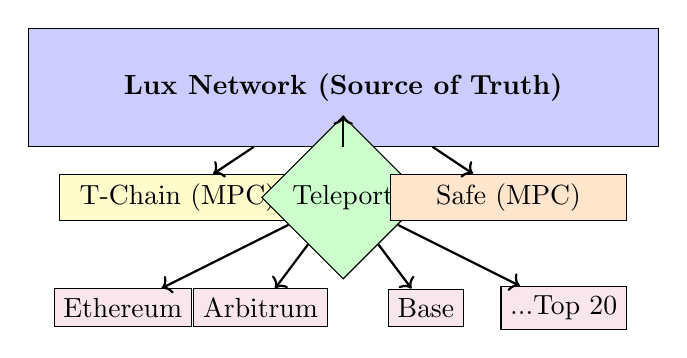
\begin{tikzpicture}[scale=0.7]
    % Lux Network (Source of Truth)
    \node[draw, rectangle, fill=blue!20, minimum width=8cm, minimum height=1.5cm] (lux) at (0,4) {
        \textbf{Lux Network (Source of Truth)}
    };

    % T-Chain (Validators + MPC)
    \node[draw, rectangle, fill=yellow!20, minimum width=3cm] (tchain) at (-3,2) {T-Chain (MPC)};

    % Teleport Bridge
    \node[draw, diamond, fill=green!20] (teleport) at (0,2) {Teleport};

    % Safe Multi-sig
    \node[draw, rectangle, fill=orange!20, minimum width=3cm] (safe) at (3,2) {Safe (MPC)};

    % Destination Chains
    \node[draw, rectangle, fill=purple!10] (eth) at (-4,0) {Ethereum};
    \node[draw, rectangle, fill=purple!10] (arb) at (-1.5,0) {Arbitrum};
    \node[draw, rectangle, fill=purple!10] (base) at (1.5,0) {Base};
    \node[draw, rectangle, fill=purple!10] (etc) at (4,0) {...Top 20};

    % Arrows
    \draw[->, thick] (lux) -- (tchain);
    \draw[->, thick] (lux) -- (teleport);
    \draw[->, thick] (lux) -- (safe);
    \draw[->, thick] (teleport) -- (eth);
    \draw[->, thick] (teleport) -- (arb);
    \draw[->, thick] (teleport) -- (base);
    \draw[->, thick] (teleport) -- (etc);
\end{tikzpicture}
\end{center}

\subsection{Warp Messaging Integration}

Lux native chains use Warp for trustless cross-chain communication:

\begin{lstlisting}[style=solidity]
interface IWarp {
    /// @notice Send cross-chain message
    function sendWarpMessage(
        bytes calldata payload
    ) external returns (bytes32 messageId);

    /// @notice Verify incoming message
    function getVerifiedWarpMessage(
        uint32 index
    ) external view returns (WarpMessage memory, bool);
}
\end{lstlisting}

\subsubsection{Message Flow}

\begin{enumerate}
    \item Source chain emits \texttt{SendWarpMessage} event
    \item Validators sign message (BLS aggregation)
    \item Relayer constructs proof (message + signatures)
    \item Destination chain verifies via precompile
    \item 67\% quorum required for validity
\end{enumerate}

\subsection{Teleport Protocol}

Teleport enables cross-chain token transfers via threshold signatures:

\begin{lstlisting}[style=rust]
pub struct TeleportTransfer {
    pub teleport_id: [u8; 32],
    pub source_chain: u64,
    pub dest_chain: u64,
    pub sender: Address,
    pub recipient: Address,
    pub amount: U256,
    pub nonce: u64,
    pub signature: Vec<u8>, // MPC threshold signature
}
\end{lstlisting}

\subsubsection{T-Chain Validator MPC}

Top validators on T-chain collectively manage Teleport:

\begin{itemize}
    \item \textbf{Key Generation}: CGGMP21 distributed keygen
    \item \textbf{Signing}: Threshold t-of-n (e.g., 67-of-100)
    \item \textbf{Verification}: Single ECDSA signature output
    \item \textbf{Key Refresh}: Proactive security without changing pubkey
\end{itemize}

\begin{center}
\begin{tabular}{lcc}
\toprule
\textbf{Operation} & \textbf{Participants} & \textbf{Output} \\
\midrule
Keygen & All validators & Shared public key \\
Sign & 67+ validators & Single signature \\
Refresh & All validators & New shares \\
\bottomrule
\end{tabular}
\end{center}

\subsection{Safe Multi-sig Management}

AI contracts are initially managed by Lux Safe (MPC wallet):

\begin{lstlisting}[style=solidity]
contract AITokenTeleport {
    /// @notice Safe multi-sig address (initial owner)
    address public safe;

    /// @notice Update Safe address (requires Safe approval)
    function setSafe(address newSafe) external onlyRole(DEFAULT_ADMIN_ROLE) {
        _grantRole(DEFAULT_ADMIN_ROLE, newSafe);
        _revokeRole(DEFAULT_ADMIN_ROLE, safe);
        safe = newSafe;
    }
}
\end{lstlisting}

\subsubsection{Safe Capabilities}

\begin{enumerate}
    \item Mint initial 10\% for LP seeding
    \item Authorize mining contracts
    \item Authorize Teleport bridge
    \item Set genesis block for mining
    \item Update treasury address
    \item Transfer admin to DAO (phase 2)
\end{enumerate}

\subsection{Initial LP Seeding}

Each chain receives one-sided LP at launch:

\begin{center}
\begin{tabular}{lccc}
\toprule
\textbf{Chain} & \textbf{AI Amount} & \textbf{Initial Price} & \textbf{Pair} \\
\midrule
Lux C-Chain & 100M & 0.0001 BTC & AI/LUX \\
Hanzo EVM & 100M & 0.0001 BTC & AI/LUX \\
Zoo EVM & 100M & 0.0001 BTC & AI/LUX \\
Ethereum & 100M & 0.0001 BTC & AI/ETH \\
Arbitrum & 100M & 0.0001 BTC & AI/ETH \\
Base & 100M & 0.0001 BTC & AI/ETH \\
... & ... & ... & ... \\
\bottomrule
\end{tabular}
\end{center}

\subsubsection{LP Setup Process}

\begin{enumerate}
    \item Safe calls \texttt{mintInitialLP(lpRecipient)}
    \item 100M AI minted to Safe/LP contract
    \item Create Uniswap V2 pair (AI/native token)
    \item Add one-sided liquidity (AI only)
    \item First swap sets initial price
\end{enumerate}

\subsection{Governance Roadmap}

\begin{center}
\begin{tabular}{lll}
\toprule
\textbf{Phase} & \textbf{Controller} & \textbf{Mechanism} \\
\midrule
1. Launch & Lux Safe (MPC) & Multi-sig approval \\
2. DAO & AI Token Holders & On-chain voting \\
3. Cross-chain & Teleport DAO & Multi-chain governance \\
\bottomrule
\end{tabular}
\end{center}

\subsubsection{Phase 1: Safe Multi-sig}

\begin{itemize}
    \item 3-of-5 or 5-of-7 threshold
    \item MPC-managed keys (no single point of failure)
    \item Time-locked critical operations
    \item Emergency pause capability
\end{itemize}

\subsubsection{Phase 2: DAO Governance}

\begin{itemize}
    \item AI token voting power
    \item Proposal + voting + timelock
    \item Parameter adjustments (treasury \%, GPU tiers)
    \item Mining contract upgrades
\end{itemize}

\subsubsection{Phase 3: Cross-chain DAO}

\begin{itemize}
    \item Votes aggregated via Teleport
    \item Unified governance across all chains
    \item Warp messages for execution
    \item Chain-specific parameters remain local
\end{itemize}

\subsection{Top 20 EVM Deployment}

\begin{center}
\begin{tabular}{lccl}
\toprule
\textbf{Chain} & \textbf{Chain ID} & \textbf{Type} & \textbf{Bridge} \\
\midrule
Lux C-Chain & 96369 & Native & Warp \\
Hanzo EVM & 36963 & Native & Warp \\
Zoo EVM & 200200 & Native & Warp \\
\midrule
Ethereum & 1 & External & Teleport \\
BSC & 56 & External & Teleport \\
Polygon & 137 & External & Teleport \\
Arbitrum & 42161 & External & Teleport \\
Optimism & 10 & External & Teleport \\
Base & 8453 & External & Teleport \\
Avalanche & 43114 & External & Teleport \\
Fantom & 250 & External & Teleport \\
Cronos & 25 & External & Teleport \\
Gnosis & 100 & External & Teleport \\
zkSync Era & 324 & External & Teleport \\
Linea & 59144 & External & Teleport \\
Scroll & 534352 & External & Teleport \\
Mantle & 5000 & External & Teleport \\
Blast & 81457 & External & Teleport \\
Mode & 34443 & External & Teleport \\
Manta & 169 & External & Teleport \\
\bottomrule
\end{tabular}
\end{center}

\subsection{Contract Addresses}

Deterministic deployment via CREATE2:

\begin{lstlisting}[style=solidity]
// Same address across all chains via CREATE2
bytes32 constant SALT = keccak256("AI_TOKEN_V1");

address token = CREATE2.deploy(
    SALT,
    type(AITokenTeleport).creationCode,
    abi.encode(safe, treasury)
);
\end{lstlisting}

\subsection{Security Properties}

\begin{enumerate}
    \item \textbf{No Single Point of Failure}: MPC/threshold throughout
    \item \textbf{Trustless Verification}: Warp + Teleport proofs
    \item \textbf{Supply Integrity}: 1B cap enforced per chain
    \item \textbf{Upgrade Safety}: Timelock on all admin operations
    \item \textbf{Cross-chain Consistency}: Lux as source of truth
\end{enumerate}

\section{Multi-Chain Deployment Guide}
\label{sec:deployment}

\subsection{Overview}

AI Token launches simultaneously on 10 EVM chains, each with independent 1B supply cap and Bitcoin-aligned mining schedule. This section details the deployment process, LP seeding, and governance setup.

\begin{center}
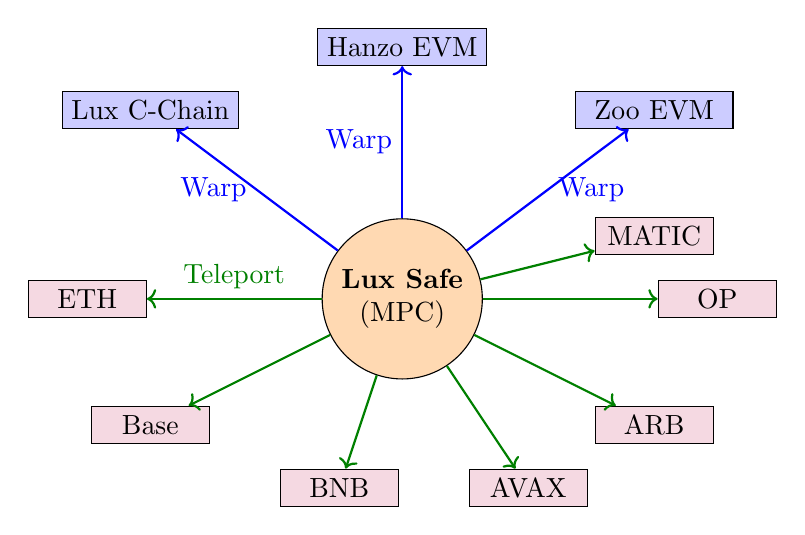
\begin{tikzpicture}[scale=0.8]
    % Central Safe
    \node[draw, circle, fill=orange!30, minimum size=2cm, align=center] (safe) at (0,0) {
        \textbf{Lux Safe}\\(MPC)
    };

    % Lux Native Chains
    \node[draw, rectangle, fill=blue!20, minimum width=2cm] (lux) at (-4,3) {Lux C-Chain};
    \node[draw, rectangle, fill=blue!20, minimum width=2cm] (hanzo) at (0,4) {Hanzo EVM};
    \node[draw, rectangle, fill=blue!20, minimum width=2cm] (zoo) at (4,3) {Zoo EVM};

    % External Chains
    \node[draw, rectangle, fill=purple!15, minimum width=1.5cm] (eth) at (-5,0) {ETH};
    \node[draw, rectangle, fill=purple!15, minimum width=1.5cm] (base) at (-4,-2) {Base};
    \node[draw, rectangle, fill=purple!15, minimum width=1.5cm] (bnb) at (-1,-3) {BNB};
    \node[draw, rectangle, fill=purple!15, minimum width=1.5cm] (avax) at (2,-3) {AVAX};
    \node[draw, rectangle, fill=purple!15, minimum width=1.5cm] (arb) at (4,-2) {ARB};
    \node[draw, rectangle, fill=purple!15, minimum width=1.5cm] (op) at (5,0) {OP};
    \node[draw, rectangle, fill=purple!15, minimum width=1.5cm] (poly) at (4,1) {MATIC};

    % Arrows from Safe
    \draw[->, thick, blue] (safe) -- (lux) node[midway, left] {Warp};
    \draw[->, thick, blue] (safe) -- (hanzo) node[midway, left] {Warp};
    \draw[->, thick, blue] (safe) -- (zoo) node[midway, right] {Warp};
    \draw[->, thick, green!50!black] (safe) -- (eth) node[midway, above] {Teleport};
    \draw[->, thick, green!50!black] (safe) -- (base);
    \draw[->, thick, green!50!black] (safe) -- (bnb);
    \draw[->, thick, green!50!black] (safe) -- (avax);
    \draw[->, thick, green!50!black] (safe) -- (arb);
    \draw[->, thick, green!50!black] (safe) -- (op);
    \draw[->, thick, green!50!black] (safe) -- (poly);
\end{tikzpicture}
\end{center}

\subsection{Deployment Sequence}

\subsubsection{Phase 1: Contract Deployment}

Deploy AIToken contract to all 10 chains using CREATE2 for deterministic addresses:

\begin{lstlisting}[style=solidity]
// Deterministic deployment via CREATE2
bytes32 constant SALT = keccak256("AI_TOKEN_V1_2025");

// Same deployer, same salt = same address on all chains
address aiToken = CREATE2.deploy(
    SALT,
    type(AIToken).creationCode,
    abi.encode(safeAddress, treasuryAddress)
);
\end{lstlisting}

\subsubsection{Deployment Order}

\begin{enumerate}
    \item \textbf{Lux Native Chains (Warp-enabled)}
    \begin{itemize}
        \item Lux C-Chain (96369) - Primary deployment
        \item Hanzo EVM (36963) - AI-focused applications
        \item Zoo EVM (200200) - Research/DeSci applications
    \end{itemize}

    \item \textbf{External EVMs (Teleport-enabled)}
    \begin{itemize}
        \item Ethereum (1) - Largest liquidity
        \item Base (8453) - Coinbase ecosystem
        \item BNB Chain (56) - High transaction volume
        \item Arbitrum (42161) - L2 scaling
        \item Optimism (10) - L2 scaling
        \item Polygon (137) - Low fees
        \item Avalanche (43114) - Fast finality
    \end{itemize}
\end{enumerate}

\subsection{Safe Multi-sig Setup}

\subsubsection{Safe Configuration}

Each chain deployment is managed by a Safe multi-sig wallet:

\begin{center}
\begin{tabular}{lcc}
\toprule
\textbf{Parameter} & \textbf{Lux Native} & \textbf{External} \\
\midrule
Threshold & 3-of-5 & 3-of-5 \\
Key Management & MPC (CGGMP21) & MPC (CGGMP21) \\
Timelock & 24 hours & 48 hours \\
Emergency Pause & 2-of-5 & 2-of-5 \\
\bottomrule
\end{tabular}
\end{center}

\subsubsection{Initial Admin Operations}

\begin{lstlisting}[style=solidity]
// 1. Deploy AIToken
AIToken token = new AIToken(safe, treasury);

// 2. Set genesis block (starts mining schedule)
token.setGenesis();

// 3. Authorize Teleport bridge
token.authorizeBridge(teleportBridge);

// 4. Authorize mining contract
token.authorizeMiner(miningContract);

// 5. Mint LP allocation to seeding address
token.mintLP(lpSeeder, 100_000_000 ether);
\end{lstlisting}

\subsection{LP Seeding Protocol}

\subsubsection{One-Sided LP Strategy}

Each chain receives 100M AI (10\%) for liquidity pool seeding at \$0.10/AI:

\begin{center}
\begin{tabular}{lccc}
\toprule
\textbf{Chain} & \textbf{AI Amount} & \textbf{Target Price} & \textbf{DEX} \\
\midrule
Lux C-Chain & 100M AI & \$0.10 & LuxSwap \\
Hanzo EVM & 100M AI & \$0.10 & HanzoSwap \\
Zoo EVM & 100M AI & \$0.10 & ZooSwap \\
Ethereum & 100M AI & \$0.10 & Uniswap V3 \\
Base & 100M AI & \$0.10 & Aerodrome \\
BNB Chain & 100M AI & \$0.10 & PancakeSwap \\
Arbitrum & 100M AI & \$0.10 & Camelot \\
Optimism & 100M AI & \$0.10 & Velodrome \\
Polygon & 100M AI & \$0.10 & QuickSwap \\
Avalanche & 100M AI & \$0.10 & Trader Joe \\
\bottomrule
\end{tabular}
\end{center}

\subsubsection{LP Pool Creation}

\begin{lstlisting}[style=solidity]
// For Uniswap V2-style DEXs
function createLP(
    address dexRouter,
    address aiToken,
    address nativeToken,
    uint256 aiAmount
) external {
    // 1. Approve router
    IERC20(aiToken).approve(dexRouter, aiAmount);

    // 2. Create pair (AI/NATIVE)
    address pair = IFactory(router.factory()).createPair(
        aiToken,
        nativeToken
    );

    // 3. Add one-sided liquidity (AI only)
    // Initial price set by first swap
    IERC20(aiToken).transfer(pair, aiAmount);
    IPair(pair).sync();
}
\end{lstlisting}

\subsubsection{Initial Price Discovery}

\begin{enumerate}
    \item Safe mints 100M AI to LP seeder contract
    \item LP seeder creates AI/NATIVE pair on DEX
    \item 50M AI deposited as one-sided liquidity
    \item First swap sets price at approximately \$0.10/AI
    \item Market discovery determines actual price
\end{enumerate}

\textbf{Target LP Composition}:
\[
\text{LP Depth} = 50\text{M AI} + \text{Native Token equivalent} \approx \$10\text{M}
\]

At \$0.10/AI:
\[
50\text{M AI} \times \$0.10 = \$5\text{M AI value}
\]

Plus matching native token:
\[
\$5\text{M ETH/BNB/etc} \rightarrow \$10\text{M total depth}
\]

\subsection{Bridge Authorization}

\subsubsection{Lux Native Chains (Warp)}

Warp messaging enables trustless cross-chain communication:

\begin{lstlisting}[style=solidity]
// No additional authorization needed
// Warp is a precompile at 0x0200...0005
// Messages verified by 67% validator quorum
\end{lstlisting}

\subsubsection{External Chains (Teleport)}

Teleport bridge requires explicit authorization:

\begin{lstlisting}[style=solidity]
// On each external chain
token.authorizeBridge(teleportBridgeAddress);

// Teleport bridge configuration
struct TeleportConfig {
    address luxEndpoint;      // Lux T-chain validator set
    uint256 threshold;        // 67-of-100 validators
    address[] validators;     // Active validator set
}
\end{lstlisting}

\subsection{Mining Contract Deployment}

\subsubsection{Mining Contract Setup}

\begin{lstlisting}[style=solidity]
contract AIMiningContract {
    AIToken public immutable aiToken;

    // Per-chain mining configuration
    uint256 public constant BLOCK_REWARD = 79.4 ether;
    uint256 public constant HALVING_INTERVAL = 6_300_000;
    uint256 public constant TREASURY_BPS = 200; // 2%

    // Mining session management
    mapping(bytes32 => Session) public sessions;

    function submitAttestation(
        bytes calldata teeQuote,
        bytes32 sessionId
    ) external {
        // Verify NVTrust TEE quote
        require(verifyTEEQuote(teeQuote), "Invalid attestation");

        // Calculate reward
        uint256 reward = calculateReward(sessionId);

        // Mint via AIToken
        aiToken.mintReward(msg.sender, reward);
    }
}
\end{lstlisting}

\subsubsection{Mining Authorization}

\begin{lstlisting}[style=solidity]
// Safe authorizes mining contract
token.authorizeMiner(miningContractAddress);

// Mining contract can now call mintReward()
\end{lstlisting}

\subsection{Genesis Block Configuration}

\subsubsection{Setting Genesis}

Genesis block marks the start of the mining schedule:

\begin{lstlisting}[style=solidity]
// Called once by Safe after deployment
token.setGenesis();

// After genesis:
// - currentEpoch() returns 0
// - currentReward() returns 79.4 AI
// - Mining can begin
\end{lstlisting}

\subsubsection{Genesis Timing}

\begin{center}
\begin{tabular}{ll}
\toprule
\textbf{Step} & \textbf{Timing} \\
\midrule
Contract deployment & Day 0 \\
Safe configuration & Day 0 \\
Bridge authorization & Day 0-1 \\
LP seeding & Day 1-2 \\
Mining contract deployment & Day 2-3 \\
Genesis block set & Day 3 (coordinated) \\
Mining begins & Day 3+ \\
\bottomrule
\end{tabular}
\end{center}

\subsection{Post-Deployment Verification}

\subsubsection{Verification Checklist}

\begin{enumerate}
    \item \textbf{Contract State}
    \begin{itemize}
        \item[$\square$] \texttt{safe} address correct
        \item[$\square$] \texttt{treasury} address correct
        \item[$\square$] \texttt{genesisBlock} set
        \item[$\square$] Bridge role granted
        \item[$\square$] Miner role granted
    \end{itemize}

    \item \textbf{LP Pools}
    \begin{itemize}
        \item[$\square$] Pair created on DEX
        \item[$\square$] LP tokens locked/burned
        \item[$\square$] Initial price approximately \$0.10
        \item[$\square$] Pool depth approximately \$10M
    \end{itemize}

    \item \textbf{Bridge}
    \begin{itemize}
        \item[$\square$] Teleport endpoints configured
        \item[$\square$] Validator set registered
        \item[$\square$] Test transfer successful
    \end{itemize}
\end{enumerate}

\subsubsection{On-Chain Verification}

\begin{lstlisting}[style=solidity]
// Verify deployment
function verify(address tokenAddress) external view returns (bool) {
    AIToken token = AIToken(tokenAddress);

    // Check constants
    require(token.LP_ALLOCATION() == 100_000_000 ether);
    require(token.MINING_ALLOCATION() == 900_000_000 ether);
    require(token.CHAIN_SUPPLY_CAP() == 1_000_000_000 ether);
    require(token.HALVING_INTERVAL() == 6_300_000);
    require(token.INITIAL_REWARD() == 79.4 ether);

    // Check state
    require(token.genesisBlock() > 0);
    require(token.safe() != address(0));
    require(token.treasury() != address(0));

    return true;
}
\end{lstlisting}

\subsection{Emergency Procedures}

\subsubsection{Pause Operations}

\begin{lstlisting}[style=solidity]
// Emergency pause (2-of-5 threshold)
function emergencyPause() external onlyEmergency {
    _pause();
    emit EmergencyPause(msg.sender, block.timestamp);
}

// Resume requires full Safe approval (3-of-5)
function unpause() external onlyRole(DEFAULT_ADMIN_ROLE) {
    _unpause();
}
\end{lstlisting}

\subsubsection{Bridge Revocation}

\begin{lstlisting}[style=solidity]
// Revoke compromised bridge
token.revokeBridge(compromisedBridge);

// Deploy new bridge with timelock
// 48-hour delay for external chains
timelockController.schedule(
    address(token),
    0,
    abi.encodeCall(token.authorizeBridge, newBridge),
    bytes32(0),
    bytes32(0),
    48 hours
);
\end{lstlisting}

\subsection{Governance Transition}

\subsubsection{Phase 1: Safe Multi-sig (Launch)}

\begin{itemize}
    \item 3-of-5 MPC-managed Safe
    \item Controls all admin functions
    \item 24-48 hour timelock on critical operations
\end{itemize}

\subsubsection{Phase 2: DAO Governance (Month 6+)}

\begin{lstlisting}[style=solidity]
// Transfer admin to DAO
function transferToDAO(address daoGovernor) external onlyRole(DEFAULT_ADMIN_ROLE) {
    // Grant admin to DAO
    _grantRole(DEFAULT_ADMIN_ROLE, daoGovernor);

    // Revoke from Safe (after DAO operational)
    // Safe retains emergency pause only
    _revokeRole(DEFAULT_ADMIN_ROLE, safe);
}
\end{lstlisting}

\subsubsection{Phase 3: Cross-chain Governance (Year 2+)}

\begin{itemize}
    \item AI token voting power across all chains
    \item Votes aggregated via Teleport/Warp
    \item Unified governance for global parameters
    \item Local parameters remain chain-specific
\end{itemize}

\subsection{Deployment Addresses}

\subsubsection{Deterministic Addresses (CREATE2)}

All contracts deployed at same address across chains:

\begin{center}
\begin{tabular}{ll}
\toprule
\textbf{Contract} & \textbf{Address (CREATE2)} \\
\midrule
AIToken & \texttt{0xAI...TOKEN} \\
Mining Contract & \texttt{0xAI...MINE} \\
LP Seeder & \texttt{0xAI...SEED} \\
Teleport Bridge & \texttt{0xAI...BRIDGE} \\
\bottomrule
\end{tabular}
\end{center}

\textit{Note: Actual addresses determined at deployment via CREATE2 with published salt.}

\subsection{Monitoring \& Analytics}

\subsubsection{Key Metrics}

\begin{enumerate}
    \item \textbf{Per-Chain Metrics}
    \begin{itemize}
        \item Total supply minted
        \item LP minted vs remaining
        \item Mining minted vs remaining
        \item Current epoch and reward
        \item Active mining sessions
    \end{itemize}

    \item \textbf{Global Metrics}
    \begin{itemize}
        \item Cross-chain total supply
        \item Teleport volume (24h, 7d, 30d)
        \item Price deviation across chains
        \item Mining hashrate equivalent
    \end{itemize}
\end{enumerate}

\subsubsection{Dashboard Endpoints}

\begin{lstlisting}[style=rust]
// Multi-chain aggregation API
GET /api/v1/ai/stats
{
    "global": {
        "total_supply": "1234567890.00",
        "total_chains": 10,
        "total_miners": 5000,
        "24h_volume": "50000000.00"
    },
    "chains": [
        {
            "chain_id": 96369,
            "name": "Lux C-Chain",
            "supply": "150000000.00",
            "price_usd": "0.12",
            "epoch": 0,
            "reward": "79.4"
        },
        // ... other chains
    ]
}
\end{lstlisting}


% Bibliography
\bibliographystyle{plain}
\bibliography{references}

\end{document}
